% $Header: /Users/joseph/Documents/LaTeX/beamer/solutions/conference-talks/conference-ornate-20min.en.tex,v 90e850259b8b 2007/01/28 20:48:30 tantau $

\documentclass{beamer}
\DeclareMathSizes{9}{8}{6}{6}

\usepackage{listings}
\usepackage{amsmath,amssymb}
\usepackage{amsthm}
\usepackage{xcolor}
%\usepackage{amsmath}
\usepackage{bm}
%\usepackage{listings}
% % \textwidth 16cm \textheight 23.5cm
% \renewcommand{\baselinestretch}{1.2}
%\usepackage{graphicx}
\usepackage{cancel}
\usepackage{graphicx}
\usepackage{floatflt,subfigure}


\input{F:/Research/Works/Templates/Mydef.tex}

% This file is a solution template for:

% - Talk at a conference/colloquium.
% - Talk length is about 20min.
% - Style is ornate.



% Copyright 2004 by Till Tantau <tantau@users.sourceforge.net>.
%
% In principle, this file can be redistributed and/or modified under
% the terms of the GNU Public License, version 2.
%
% However, this file is supposed to be a template to be modified
% for your own needs. For this reason, if you use this file as a
% template and not specifically distribute it as part of a another
% package/program, I grant the extra permission to freely copy and
% modify this file as you see fit and even to delete this copyright
% notice. 


\mode<presentation>
{
  \usetheme{Warsaw}
  % or ...

  \setbeamercovered{transparent}
  % or whatever (possibly just delete it)
}


\usepackage[english]{babel}
% or whatever

\usepackage[latin1]{inputenc}
% or whatever

\usepackage{times}
\usepackage[T1]{fontenc}
% Or whatever. Note that the encoding and the font should match. If T1
% does not look nice, try deleting the line with the fontenc.


\title[Collective Emission Studies Using Green Function Method] % (optional, use only with long paper titles)
{Collective Emission Studies\\ Using Green Function Method}

%\subtitle
%{Based on Green Function Method and Photonic Simulations}

\titlegraphic{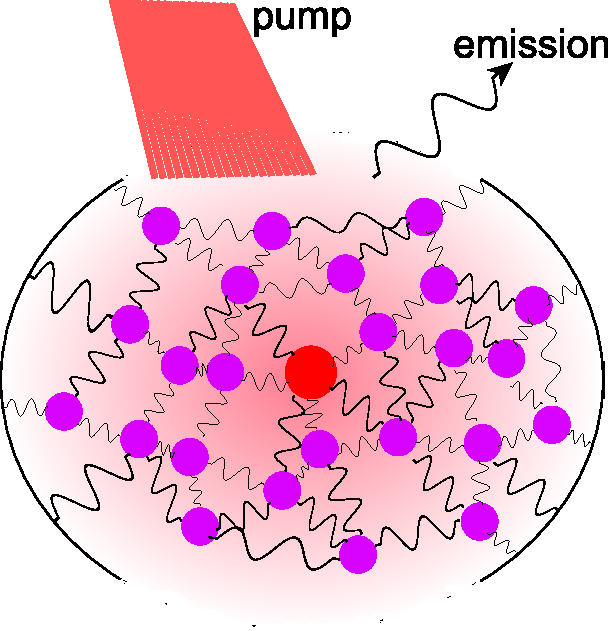
\includegraphics[width=.15\textwidth]{./Figs/Cavity_pump}}

\author[Xiaodong Qi] % (optional, use only with lots of authors)
{Xiaodong Qi} %\inst{1}}
% - Give the names in the same order as the appear in the paper.
% - Use the \inst{?} command only if the authors have different
%   affiliation.

\institute[Universities of New Mexico] % (optional, but mostly needed)
{
  %\inst{1}%
  Department of Physics and Astronomy, Universities of New Mexico
  }
% - Use the \inst command only if there are several affiliations.
% - Keep it simple, no one is interested in your street address.

\date[Jan, 2013] % (optional, should be abbreviation of conference name)
{CQuIC Presentation, Jan, 2013}
% - Either use conference name or its abbreviation.
% - Not really informative to the audience, more for people (including
%   yourself) who are reading the slides online

\subject{Theoretical Study on Quantum Optics}
% This is only inserted into the PDF information catalog. Can be left
% out. 



% If you have a file called "university-logo-filename.xxx", where xxx
% is a graphic format that can be processed by latex or pdflatex,
% resp., then you can add a logo as follows:

% \pgfdeclareimage[height=0.5cm]{university-logo}{university-logo-filename}
% \logo{\pgfuseimage{university-logo}}



% Delete this, if you do not want the table of contents to pop up at
% the beginning of each subsection:
\AtBeginSubsection[]
{
  \begin{frame}<beamer>{Outline}
    \tableofcontents[currentsection,currentsubsection]
  \end{frame}
}


% If you wish to uncover everything in a step-wise fashion, uncomment
% the following command: 

%\beamerdefaultoverlayspecification{<+->}


\begin{document}

\begin{frame}
%   \tikz [remember picture,overlay]
%    {\node at
%        ([yshift=3cm]current page.south) 
%        %or: (current page.center)
%        {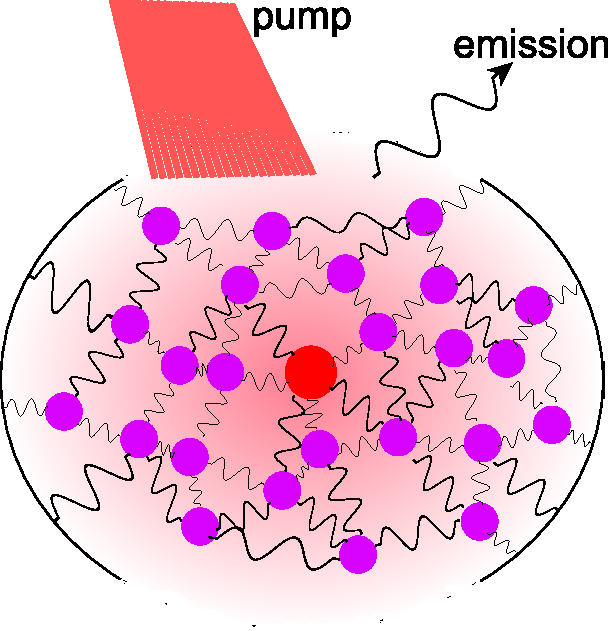
\includegraphics[width=.5\textwidth]{./Figs/Cavity_pump}};}
  \titlepage
\end{frame}

\begin{frame}{Outline}
  \tableofcontents
  % You might wish to add the option [pausesections]
\end{frame}


% Structuring a talk is a difficult task and the following structure
% may not be suitable. Here are some rules that apply for this
% solution: 

% - Exactly two or three sections (other than the summary).
% - At *most* three subsections per section.
% - Talk about 30s to 2min per frame. So there should be between about
%   15 and 30 frames, all told.

% - A conference audience is likely to know very little of what you
%   are going to talk about. So *simplify*!
% - In a 20min talk, getting the main ideas across is hard
%   enough. Leave out details, even if it means being less precise than
%   you think necessary.
% - If you omit details that are vital to the proof/implementation,
%   just say so once. Everybody will be happy with that.

\section{Theory of Green Function Method in Nanophotonics}

\subsection{Initial Motivation}

\begin{frame}{Initial motivation}
  % - A title should summarize the slide in an understandable fashion
  %   for anyone how does not follow everything on the slide itself.
\begin{columns}
 \column{0.5\textwidth}
  \begin{itemize}
  \item
    Research Background.
  \item
    Simulation Difficulty.
  \item
    Inspired Paper: \\ M. Wubs, \textit{Phys. Rev. A.}, 2004, \textit{70, 053823}.
  \end{itemize}
 
 \column{0.5\textwidth}
  \begin{figure}[htp]%[floatfix]
  \centering
  \begin{center}
 %\DeclareGraphicsRule{.pdf}{eps}{}{`convert #1 eps:-}
  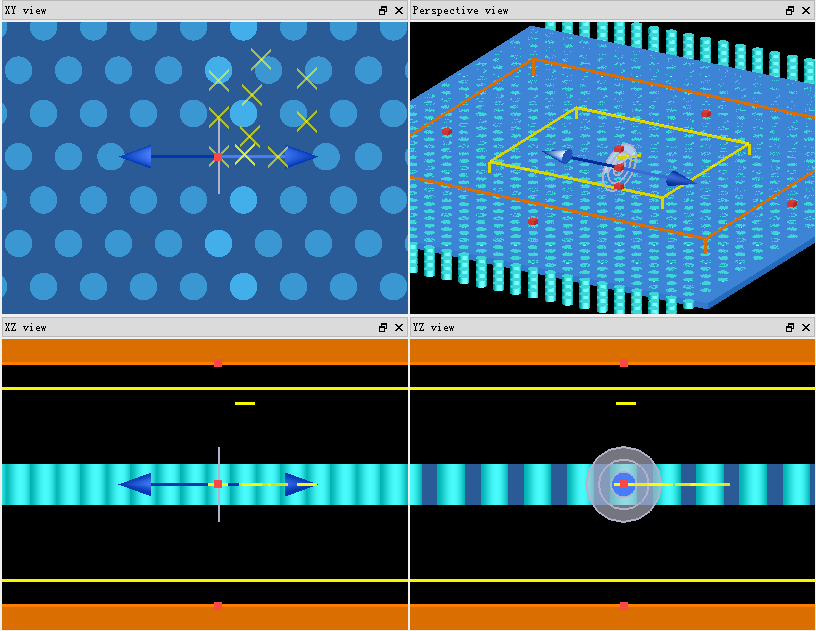
\includegraphics[width=6cm]{./Figs/FDTDsimulation}%[bb=1.0in 1.0in 7.5in 10in]
  \end{center}
  \caption[An FDTD simulation diagram of a H3 PC cavity.]{An FDTD simulation diagram of a H3 PC cavity.}
  \label{FDTDsimulation}
  \end{figure}
\end{columns}
\end{frame}

\subsection{Study Objects in Nanophotonics}

\begin{frame}{Cavity Model}
\begin{columns}
\column{0.4\textwidth}
 \begin{figure}[htp]%[floatfix]
  \centering
 \begin{center}
 %\DeclareGraphicsRule{.pdf}{eps}{}{`convert #1 eps:-}
 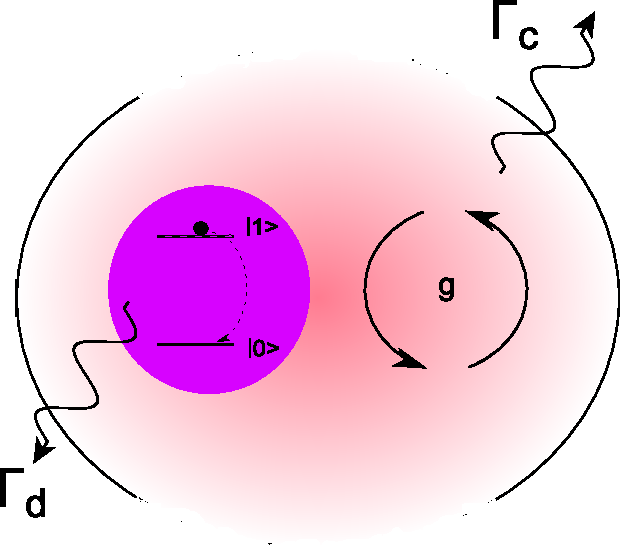
\includegraphics[width=0.99\textwidth]{./Figs/Cavity_withDipoleT}%[bb=1.0in 1.0in 7.5in 10in]
 \end{center}
 \caption[A diagram of a cavity with one dipole.]{A diagram of a cavity with one dipole. }
 \label{Cavity_withDipoleT1}
 \end{figure}

\column{0.6\textwidth}
\begin{center} %{Dipole momentum}
\fontsize{9}{7.2}\selectfont
%\scalebox{0.5}{
{Dipole momentum: 
 \begin{align}
 \hat{\mathbf{d}}(t) &={\bm \mu_d}[\hat{\sigma}_d^-(t=0) e^{-i(\Omega_d-i\Gamma_d/2) t}\nonumber \\
 &\quad\quad  +\hat{\sigma}_d^+(t=0)e^{i(\Omega_d+i\Gamma_d/2) t}],\label{eq:dt2}
 \end{align}
or
 \begin{align}
  \label{dipole}
   \hat{\mathbf{d}}(\omega) &=
 {i\bm\mu_d}\left [ \frac{\hat{\sigma}_d^-(t=0)}
 {\omega-\Omega_d+i\Gamma_d/2}\nonumber \right. \\ &\qquad\quad \left. +\frac{\hat{\sigma}_d^+(t=0)}{\omega+\Omega_d+i\Gamma_d/2}\right].
 \end{align}
 }
\end{center}
\end{columns}

%  You can create overlays\dots
%  \begin{itemize}
%  \item using the \texttt{pause} command:
%    \begin{itemize}
%    \item
%      First item.
%      \pause
%    \item    
%      Second item.
%    \end{itemize}
%  \item
%    using overlay specifications:
%    \begin{itemize}
%    \item<3->
%      First item.
%    \item<4->
%      Second item.
%    \end{itemize}
%  \item
%    using the general \texttt{uncover} command:
%    \begin{itemize}
%      \uncover<5->{\item
%        First item.}
%      \uncover<6->{\item
%        Second item.}
%    \end{itemize}
%  \end{itemize}

\end{frame}


\subsection{Green Function of An Optical Cavity Coupled to $N$ Excitons }

\begin{frame}{Hamiltonian and LS Equations}
Cavity-exciton Hamiltonian in the absence of dephasing and decoherence:
\begin{equation}
\label{eq:h}
\begin{split}
 \hat{H} =& \hat{H}_{X}+\hat{H}_F+\hat{H}_I\\
=& \sum_n\! \hbar \Omega_n \hat{\sigma}_n^+\hat{\sigma}_n^- \! +\!
\sum_\lambda\! \hbar \omega_\lambda
\hat{a}_\lambda^\dagger\hat{a}_\lambda \nonumber +\! \sum_{n,\lambda}\! (
\hat{\sigma}_n^- + \hat{\sigma}_n^+)(g_{n\lambda}
\hat{a}_\lambda+g_{n\lambda}^*\hat{a}_\lambda^\dagger),\\
\end{split}
\end{equation}
where the coupling strength is 
\begin{equation}
g_{n\lambda}=-i\sqrt{\frac{\hbar\omega_\lambda}{2 \varepsilon_0}}\boldsymbol{\mu}_n\cdot \mathbf{f}_\lambda(\mathbf{r}_n).
\end{equation}
\end{frame}

\begin{frame}{Hamiltonian and LS Equations}
The Heisenberg equations of motion for the operators can be derived from  $\dot { O}_i = -i{\hbar^{-1}[ O_i,H]}$,
yielding
\begin{align}
\frac{d\hat{a}_\lambda}{dt}&=-i\omega_\lambda \hat{a}_\lambda-i\sum_n\hbar^{-1}g_{n\lambda}^*(\hat{\sigma}_n^-+\hat{\sigma}_n^+), \label{eq:a-t}\\
%
\frac{d\hat{a}_\lambda^\dagger}{dt}&=i\omega_\lambda \hat{a}_\lambda^\dagger+i\sum_n\hbar^{-1}g_{n\lambda}(\hat{\sigma}_n^-+\hat{\sigma}_n^+), \label{eq:a+t}\\
%
\frac{d\hat{\sigma}_n^-}{dt}&=-i\Omega_n\hat{\sigma}^-_n-i\hbar^{-1}\sum_{\lambda}(g_{n\lambda}
\hat{a}_\lambda+g_{n\lambda}^*\hat{a}_\lambda^\dagger), \label{eq:sig-t} \\
%
\frac{d\hat{\sigma}_n^+}{dt}&=i\Omega_n\hat{\sigma}^+_n+i\hbar^{-1}\sum_{\lambda}(g_{n\lambda}
\hat{a}_\lambda+g_{n\lambda}^*\hat{a}_\lambda^\dagger). \label{eq:sig+t}
%
%\frac{d\hat{\sigma}_{nz}}{dt}&=2i\hbar^{-1}\sum_{\lambda}(\hat{\sigma}_n^-- %\hat{\sigma}_n^+)(g_{n\lambda}
%\hat{a}_\lambda+g_{n\lambda}^*\hat{a}_\lambda^\dagger).
\end{align}
\end{frame}

\begin{frame}{Hamiltonian and LS Equations}
Next we perform a Laplace transform to positive frequency space,
$O(\omega)=\int_0^\infty \drv t\, e^{i\omega t}\, O(t)$, and obtain:
\begin{center}
\fontsize{7.8}{-0.2}\selectfont
\begin{align}
{\hat{a}_\lambda(\omega)}&= \hat{a}_\lambda(t=0) + \frac{i\hbar^{-1}}{\omega-\omega_\lambda}
\sum_n g_{n\lambda}^*[\frac{\hat{\sigma}_n^-(t=0)}{\omega-\omega_\lambda}
+\frac{\hat{\sigma}_n^+(t=0)}{\omega+\omega_\lambda}]\nonumber\\
& \quad + \frac{\hbar^{-2}}{\omega-\omega_\lambda}
\sum_{n,\lambda'} \frac{2g_{n\lambda}^*\Omega_n}{\omega^2-\Omega_n^2} [g_{n\lambda'}
\hat{a}_{\lambda'}(\omega)+g_{n\lambda'}^*\hat{a}_{\lambda'}^\dagger(\omega)], \label{eq:aw} \\
{\hat{a}_\lambda^\dagger(\omega)}&=\adag_\lambda(t=0) - \frac{i\hbar^{-1}}{\omega-\omega_\lambda}
\sum_n g_{n\lambda}^*[\frac{\hat{\sigma}_n^-(t=0)}{\omega-\omega_\lambda}
-\frac{\hat{\sigma}_n^+(t=0)}{\omega+\omega_\lambda}]\nonumber\\
& \quad + \frac{\hbar^{-2}}{\omega+\omega_\lambda}
\sum_{n,\lambda'} \frac{2g_{n\lambda}\Omega_n}{\omega^2-\Omega_n^2} [g_{n\lambda'}
\hat{a}_{\lambda'}(\omega)+g_{n\lambda'}^*\hat{a}_{\lambda'}^\dagger(\omega)],
\label{eq:adaggerw} \\
\hat{\sigma}_n^-(\omega)&=\frac{i\hat{\sigma}_n^-(t=0)}
{\omega-\Omega_n}+\frac{\hbar^{-1}}{\omega-\Omega_n}
\sum_{\lambda}[g_{n\lambda}
\hat{a}_\lambda(\omega)+g_{n\lambda}^*\hat{a}_\lambda^\dagger(\omega)], \label{eq:sig-w} \\
\hat{\sigma}_n^+(\omega)&=\frac{i\hat{\sigma}_n^+(t=0)}
{\omega+\Omega_n}-\frac{\hbar^{-1}}{\omega+\Omega_n} \sum_{\lambda}[g_{n\lambda}
\hat{a}_\lambda(\omega)+g_{n\lambda}^*\hat{a}_\lambda^\dagger(\omega)]. \label{eq:sig+w}
%\hat{\sigma}_{nz}(\omega)&=\frac{i\hat{\sigma}_{nz}(t=0)}
%{\omega}+\frac{2\hbar^{-1}\mu_n\hat{E}_\mu(\mathbf{r}_n)\ast
%[\hat{\sigma}_{n}^-(\omega)-\hat{\sigma}_{n}^+(\omega)]}{\omega}.
\end{align}
\end{center}
\end{frame}

\begin{frame}{Hamiltonian and LS Equations}
\fontsize{9}{-0.2}\selectfont
Using
\begin{equation}
 \label{eq:Esum}
 \hat{\mathbf{E}}(\mathbf{r})=\hat{\mathbf{E}}^+(\mathbf{r})+\hat{\mathbf{E}}^-(\mathbf{r})=i\sum_\lambda\sqrt{\frac{\hbar
\omega_\lambda}{2\varepsilon_0}}\hat{a}_\lambda\mathbf{f}_\lambda(\mathbf{r})+h.c.
\end{equation}
we obtain the Lippmann-Schwinger equation for the field operator
\begin{subequations}
\label{eq:ew1_1}
\begin{align}
\hat{\mathbf{E}}(\mathbf{r},\omega) =& \hat{\mathbf{E}}^{(0)}(\mathbf{r},\omega)\label{bareE0_1}\\
&+ \sum_n{\mathbf{K}(\mathbf{r},\mathbf{r}_n,\omega)\cdot\hat{\mathbf{S}}_n(\omega)}\label{sourceE_1}\\
&+ \sum_n{\mathbf{K}(\mathbf{r},\mathbf{r}_n,\omega)\cdot\mathbf{U}_n(\omega)\cdot\hat{\mathbf{E}}(\mathbf{r}_n,\omega)}\label{scatteringE_1}
\end{align}
\end{subequations}
%
\begin{equation}
 =\hat{\mathbf{E}}^{(0)}(\mathbf{r},\omega)+ \hat{\mathbf{E}}_{source}(\mathbf{r},\omega) +\hat{\mathbf{E}}_{scatt}(\mathbf{r},\omega)\label{eq:E0sourcescatt_1}.
% This is an important equation.
\end{equation}
\end{frame}

\begin{frame}{Hamiltonian and LS Equations}
\begin{columns}
\column{0.4\textwidth}
\fontsize{6.8}{-0.2}\selectfont
\begin{subequations}
\begin{align}
\hat{\mathbf{E}}(\mathbf{r},\omega) =& \hat{\mathbf{E}}^{(0)}(\mathbf{r},\omega)\nonumber \\
&+ \color{purple}{\sum_n{\mathbf{K}(\mathbf{r},\mathbf{r}_n,\omega)\cdot\hat{\mathbf{S}}_n(\omega)}}\nonumber \\
&+\color{blue}{ \sum_n{\mathbf{K}(\mathbf{r},\mathbf{r}_n,\omega)\cdot\mathbf{U}_n(\omega)\cdot\hat{\mathbf{E}}(\mathbf{r}_n,\omega)}}\nonumber
\end{align}
\end{subequations}
%
\begin{equation}
 =\hat{\mathbf{E}}^{(0)}(\mathbf{r},\omega)+ \color{purple}{\hat{\mathbf{E}}_{source}(\mathbf{r},\omega)} +\color{blue}{\hat{\mathbf{E}}_{scatt}(\mathbf{r},\omega)}. \nonumber
% This is an important equation.
\end{equation}

\begin{figure}[htp]%[floatfix]
  \centering
 \begin{center}
 %\DeclareGraphicsRule{.pdf}{eps}{}{`convert #1 eps:-}
 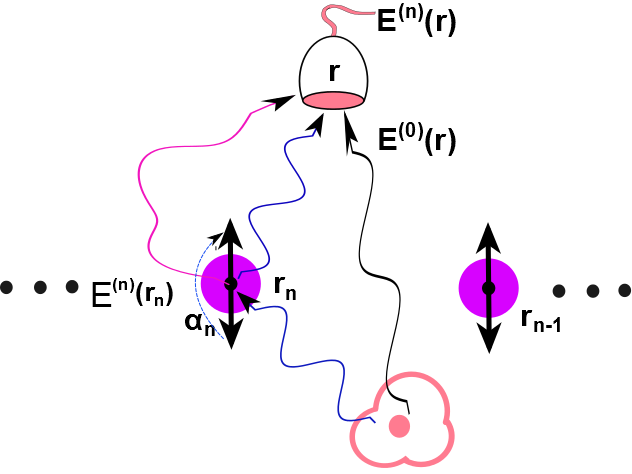
\includegraphics[width=0.98\textwidth]{./Figs/EDetection}%[bb=1.0in 1.0in 7.5in 10in]
 \end{center}
 %\caption[A diagram of E.]{\fontsize{6.5}{-0.2}\selectfont A diagram of $\mathbf{E}$. }
 \label{EDetection}
 \end{figure}

\column{0.6\textwidth}
\fontsize{6.8}{-0.2}\selectfont
\textbf{Wub's Green function} (no-decay form):
\begin{equation}
 \label{K}
 \mathbf{K}(\mathbf{r},\mathbf{r}',\omega)=c^2\sum_\lambda \mathbf{f}_\lambda(\mathbf{r})\mathbf{f}_\lambda^*(\mathbf{r}')\omega_\lambda^2\left[ \frac{1}
{(\omega^2-\omega_\lambda^2){\omega^2}}+1 \right].\nonumber
\end{equation}
\textcolor{purple}{Source operator}:
\begin{align}
 \label{source}
 \color{purple}{\hat{\mathbf{S}}_n(\omega)} &\color{purple}{\equiv \left(\frac{i{\bm \mu}_n\omega^2}{\varepsilon_0c^2}\right)
\lbrack\frac{\hat{\sigma}_n^-(t=0)}{\omega-\Omega_n}+\frac{\hat{\sigma}_n^+(t=0)}{\omega+\Omega_n}\rbrack} \nonumber\\
&\color{purple}{=\frac{\omega^2}{\varepsilon_0c^2}\hat{\mathbf{d}}_n(\omega)}.\nonumber  
\end{align}
\textcolor{blue}{Optical potential tensors}:
\begin{equation}
 \label{Un}
\color{blue}{ \mathbf{U}_n(\omega) \equiv \left(\frac{\mu_n^2\omega^2}{\hbar\varepsilon_0c^2}\right)
\left(\frac{2\Omega_n}{\Omega_n^2-\omega^2}\right)\mathbf{e}_n \otimes \mathbf{e}_n=\frac{\omega^2}{c^2}{\bm \alpha}_n(\omega)}. \nonumber
\end{equation}

\end{columns}
\end{frame}

%\begin{frame}{Hamiltonian and LS Equations}
%
%\end{frame}

\begin{frame}{Wub's GF $\mathrm{K}(\rr,\omega)$ and Classical GF $\mathrm{G}(\rr,\omega)$}
According to Wubs's work, there are simple relationships among the quantum Green function tensor, $\Krrw$, 
%the classical transverse Green function tensor, $\GTrrw$, 
and the classical total Green function, $\Grrw$:
\begin{equation}
 \label{KG}
 \Krrw=\Grrw+\frac{\mathbf{I}\delta(\mathbf{r}-\mathbf{r}')}{\varepsilon(\mathbf{r})(\omega/c)^2}
\approx \Grrw, \nonumber %=\GTrrw+\frac{\bm{\delta}^T(\rr)}{\varepsilon(\mathbf{r})(\omega/c)^2},\nonumber
\end{equation}
where $\mathbf{I}$ is the unit dyadic. 
%, and $\bm{\delta}^T(\rr)
%=\sum_\lambda{\mathbf{f}_{\lambda}(\mathbf{r})\mathbf{f}_{\lambda}^*(\mathbf{r}')}\varepsilon(\mathbf{r})$
%is a generalized transverse delta function.
\end{frame}

\begin{frame}{Classical GF $\mathrm{G}(\rr,\omega)$ and FDTD method}
\fontsize{9}{-0.2}\selectfont
A GF corresponding to an E-field of $\mathbf{f}(\mathbf{r})$ is defined in the form of a wave equation with a dipole source (a delta function):
\begin{equation}
\label{def:GEwave}
 -\nabla \times \nabla \times \mathbf{G}(\rr,\omega) + \varepsilon(\mathbf{r})(\omega/c)^2 \mathbf{G}(\rr,\omega) = \mathbf{I} \delta \left(\br-\br'\right).\nonumber
\end{equation}
The GF defined above describes how the wave propagates from the source $\mathbf{r}'$ to a detector at $\mathbf{r}$.

If the background E-field at $\br$ is $\mathbf{E}_0$, then the E-field at $\br$ responding to a polarized source at $\br'$ is given by
\begin{equation}
 \label{EandGwithE0}
\mathbf{E}(\mathbf{r})=\mathbf{E}_0(\mathbf{r
})+\mathbf{G}(\mathbf{r},\mathbf{r}') \cdot \mathbf{P}(\mathbf{r}'),
\end{equation}
where $\mathbf{P}$ is the source's polarization vector or polarization density.
Now, we let $\mathbf{E}_0=0$, which means there is no initial E-field at the detector's position.
Hence, one has
\begin{equation}\label{eq:EGP}
\mathbf{E}(\mathbf{r})=\mathbf{G}(\mathbf{r},\mathbf{r}') \cdot \mathbf{P}(\mathbf{r}').
\end{equation}
\end{frame}

\begin{frame}{Classical GF $\mathrm{G}(\rr,\omega)$ and FDTD method}
\fontsize{8}{-0.2}\selectfont
In terms of matrices
\begin{align}
\label{EandGwithoutE0}
\left( \begin{array}{c}
       E_x\\
       E_y\\
       E_z  \end{array} \right)
                   = \left( \begin{array}{c}
                      G_{xx} \quad G_{xy} \quad G_{xz} \\
                      G_{yx} \quad G_{yy} \quad G_{yz} \\
                      G_{zx} \quad G_{zy} \quad G_{zz}  \end{array}  \right) \left( \begin{array}{c}
                                                                                     P_x\\
                                                                                     P_y\\
                                                                                     P_z
                                                                                    \end{array} \right).\nonumber
\end{align}
If we let the polarization source only have $x$ component or orientate the polarized source to $x$ direction, which means
\begin{equation}
 \label{Px}
\mathbf{P}=\left( \begin{array}{c}
                   P_x\\
                   0\\
                   0
                  \end{array} \right),
\end{equation}
then only the first column of GF contributes to the measured E-field, and we obtain
\begin{equation}
 \label{Gix}
G_{ix} \equiv \frac{E_{i}}{P_x}, \quad (i=x, y, z).
\end{equation}
The $G_{ix}\,(i=x, y, z)$ stretch out the first column of the GF. Similarly, we can obtain the other elements of the GF. 
\end{frame}


\begin{frame}{Classical GF $\mathrm{G}(\rr,\omega)$ and FDTD method}
\begin{columns}
\column{0.4\textwidth}

 \begin{figure}[htp]%[floatfix]
  \centering
 \begin{center}
 %\DeclareGraphicsRule{.pdf}{eps}{}{`convert #1 eps:-}
 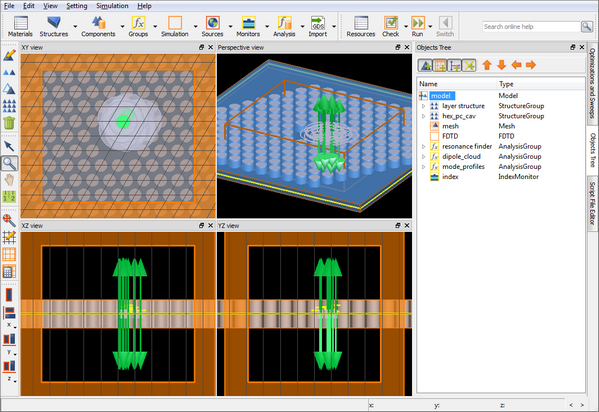
\includegraphics[width=0.99\textwidth]{./Figs/pc_3d_cavity_pc}%[bb=1.0in 1.0in 7.5in 10in]
 \end{center}
 \caption[A diagram of FDTD simulation setting.]{\fontsize{8}{-0.2}\selectfont Dipole sources in an FDTD Solutions interface. }
 \label{Cavity_FDTD_Source}
 \end{figure}
 
\column{0.6\textwidth}
\fontsize{8}{-0.2}\selectfont
%The FDTD method is a numerical method to calculate the time domain electromagnetic field propagating in an arbitrary optical structure.

The background GF tensor components can be calculated through
\begin{equation}
 \label{def:GFT}
 G_{ij}(\rr,\omega)=\frac{{\rm FT}[E^i_\lambda(\mathbf{r},t)]}{{\rm FT}[E^j_d(\mathbf{r}',t)]}
=\frac{E^i_\lambda(\mathbf{r},\omega)}{E^j_d(\mathbf{r}',\omega)}, \quad (i,j=x, y, z),\nonumber
\end{equation}
where we assume the test dipole source is located at $\mathbf{r}'$ and only has a $j$ component of polarized electric field $P^j(\mathbf{r}')=E^j_d(\mathbf{r}')$, ${\rm FT}$ indicates Fourier transformation.

\end{columns}
\end{frame}

\begin{frame}{Classical GFs in a Cavity}
\fontsize{9}{-0.2}\selectfont
For a typical optical cavity coupling with QDs, one can have the analytical GF given by
\begin{equation}
 \label{Ganal}
\mathbf{G}=\mathbf{G}_{cav}+\mathbf{G}_{eva}\approx \mathbf{G}_{cav},
\end{equation}
\begin{equation}
 \label{Gcav}
\mathbf{G}_{cav}(\br,\br',\omega)=\sum_{c\lambda}{\frac{\omega^2\mathbf{f}_{c\lambda}(\mathbf{r},\omega_{c\lambda})\mathbf{f}_{c\lambda}^*(\mathbf{r}',\omega_{c\lambda})}
{\omega_{c\lambda}^2-\omega^2-i\omega\Gamma_{c\lambda}}},
\end{equation}
where $\mathbf{G}_{eva}$ is the evanescent GF, which usually does not have an explicit analytical expression; $c\lambda$ denote the modes of the cavity, $\Gamma_{c\lambda}$ is the decay rate~\footnote{Generally, to include decay or loss (characterized by $\Gamma_n$), we can simply add a phenomenological decay constant to the resonance energies of the lossless formulas, i.e.
$\omega \pm \Omega_n \rightarrow \omega\pm \Omega_n +
i\Gamma_n/2$, and $\omega^2- \Omega_n^2+
i\omega\Gamma_n$.\label{fn:decayrevision}} or FWHM of cavity mode $\mathbf{f}_{c\lambda}(\omega)$.
\end{frame}

\begin{frame}{Classical GFs in a Cavity}
\fontsize{9}{-0.2}\selectfont
Note that, in the linear optics of dielectric material, we have
\begin{equation}
\mathbf{P}=\varepsilon_0\mathbf{\chi} \cdot \mathbf{E},
\end{equation}
or
\begin{equation}\label{eq:polarization}
\mathbf{E}=\frac{1}{\varepsilon_0}\mathbf{\chi}^{-1} \cdot \mathbf{P},
\end{equation}
where $\mathbf{\chi}$ is the electric susceptibility of the medium.
By comparing $\mathbf{E}(\mathbf{r}')=\mathbf{G}(\mathbf{r}',\mathbf{r}') \cdot \mathbf{P}(\mathbf{r}')$ with the linear polarization equation above, one can find that 
\begin{equation}
\mathbf{G}\equiv \frac{1}{\varepsilon_0}\mathbf{\chi}^{-1}.
\end{equation}
This relationship above shows that the GF method only works in linear optics regime, and can indicate optical properties of optical structures.
\end{frame}

\begin{frame}{Calculation of GFs}
Now, the E-field operator can be represented as
\begin{align}
 \hat{\mathbf{E}}^{(N)}(\mathbf{r},\omega) &=\E0+\frac{1}{\varepsilon_0}\sum_{n=1}^N{\mathbf{G}^{(0)}(\rrn,\omega)\cdot \hat{\mathbf{d}}_n(\omega)} \nonumber \\
 &\quad +\sum_{n=1}^N{\mathbf{G}^{(0)}(\rrn,\omega)\cdot \Alphanw \cdot \hat{\mathbf{E}}^{(N)}(\mathbf{r}_n,\omega)},  \label{E4GNS}
\end{align}

\end{frame}

\begin{frame}{Calculation of GFs}
\fontsize{9}{-0.2}\selectfont
In the case of  $\E0=0$, we have
\begin{align}
 \label{E4GNS_0}
 \hat{\mathbf{E}}^{(N)}(\mathbf{r},\omega) &=\frac{1}{\varepsilon_0}\sum_{n=1}^N{\mathbf{G}^{(0)}(\rrn,\omega)\cdot \hat{\mathbf{d}}_n(\omega)} \nonumber \\
 &\quad +\sum_{n=1}^N{\mathbf{G}^{(0)}(\rrn,\omega)\cdot \Alphanw \cdot \hat{\mathbf{E}}^{(N)}(\mathbf{r}_n,\omega)}.
\end{align}
The implicit scattering type formulation of Equ.\eqref{E4GNS_0} suggests that one can rewrite it in an explicit form as
\begin{equation}
 \label{E4GNS_1}
\Erw =\frac{1}{\varepsilon_0}\sum_{n=1}^N{\mathbf{G}^{(N)}(\rrn,\omega)\cdot \hat{\mathbf{d}}_n(\omega)},
\end{equation}
where $\GN(\rr,\omega)$ contains the scattering properties
of all $N$ excitons in the sample. 
\end{frame}

\begin{frame}{Calculation of GFs}
\fontsize{9}{-0.2}\selectfont
$\GN(\rr,\omega)$ formally is the self-consistent solution to the Dyson equation in the form
\begin{equation}
 \label{dysonGN}
\GN(\rr,\omega)=\mathbf{G}^0(\rr,\omega)+\sum_{n=1}^N{\mathbf{G}^0(\rrn,\omega)\cdot \Alphanw \cdot \GN(\mathbf{r}_n,\mathbf{r}',\omega)}.
\end{equation}
In a iterative scheme, it gives a series of iterative Dyson equations{\footnote{Martin,\textit{J. Opt. Soc. Am. A, OSA,} \textbf{1994}, \textit{11, 1073-1080.}}} as
\begin{equation}
 \label{dysonGn}
\Gn(\rr)=\Gm1(\rr)+{\Gm1(\rrn)\cdot {\bm \alpha}_n \cdot \Gn(\mathbf{r}_n,\mathbf{r}')}.
\end{equation}
for $1 \leq  n \leq  N$.
\end{frame}

\begin{frame}{Calculation of GFs}
\begin{columns}
\column{0.4\textwidth}
\begin{figure}[h]%[floatfix]
\centering
\begin{center}
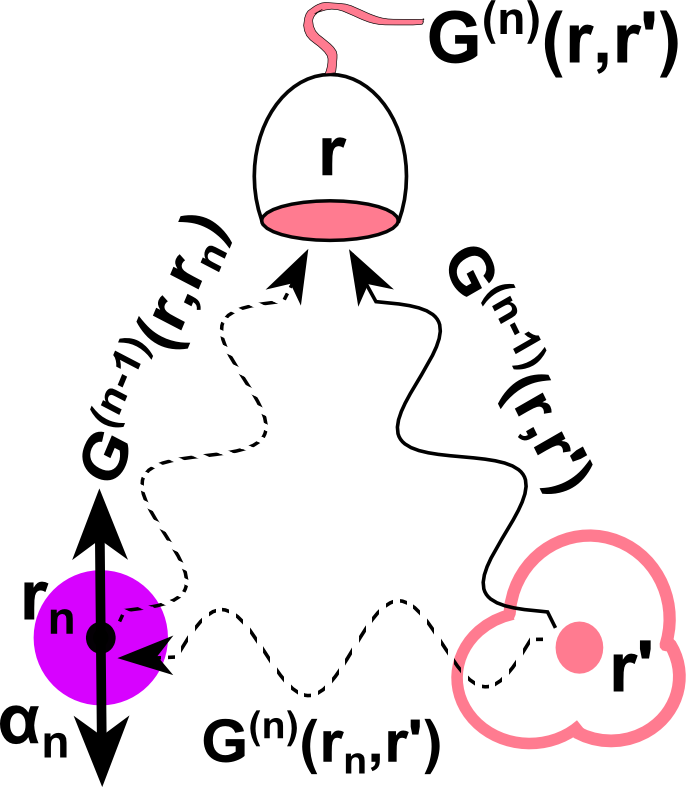
\includegraphics[width=0.9\textwidth]{./Figs/GnDetection}%[bb=1.0in 1.0in 7.5in 10in]
\end{center}
\caption[The physics picture of Dyson equations.]{The physics picture of the $n$-th order Dyson equations for $\Gn(\rr)$. }
%\label{GnDetection}
\end{figure}
\column{0.6\textwidth}
To solve the series of equation, we first make $\mathbf{r}=\mathbf{r}_i$, and iterate from the $n=1$ order of the equations
\begin{align}
%\label{dysonGnij}
\Gn(\mathbf{r}_i,\mathbf{r}_j) &=\Gm1(\mathbf{r}_i,\mathbf{r}_j)\nonumber \\ 
&\quad +{\Gm1(\mathbf{r}_i,\mathbf{r}_n)\cdot {\bm \alpha}_n\cdot \Gn(\mathbf{r}_n,\mathbf{r}_j)}.\nonumber
\end{align}

Then we can obtain $\Gn(\mathbf{r},\mathbf{r}_j)$ detected at arbitrary positions.
\end{columns}
\end{frame}


%\begin{frame}{Some special cases}

%\end{frame}



\begin{frame}{Emission and Spectrum}
By definition, the emission power spectrum is given by
\begin{align}
 \label{spectrumdef}
S(\mathbf{r},\omega) =& \int_0^\infty \!\! \int_0^\infty\!\!
\mathrm{d}t_1\mathrm{d}t_2 \, e^{i\omega(t_2-t_1)}\mathinner{\langle}\hat{\mathbf{E}}^-(t_1)\hat{\mathbf{E}}^+(t_2)\mathinner{\rangle} \\
=& \langle
(\hat{\mathbf{E}}(\omega))^{\dagger}\hat{\mathbf{E}}(\omega)\rangle\\
=& \left|\mathbf{E}^{(N)}(\br,\omega)\right|^2,
\end{align}
where
\begin{equation}
 \left| \mathbf{E}^{(N)}(\br,\omega)\right| =\frac{1}{\varepsilon_0}\langle \sum_n{\GN(\rrn,\omega)\cdot \mathbf{d}_n(\omega)}\rangle.
\end{equation}
\end{frame}

\begin{frame}{Emission and Spectrum}
\fontsize{9}{-0.2}\selectfont
If we only excite one dipole to form an initial mixed state indicated by
\begin{equation}
\rho=\frac{1}{N}\eye,
\end{equation}
where $\eye$ is a $N\times N$ diagonal unit matrix, the spectrum is given by 
\begin{align}
S({\bf r},\omega)&=\frac{1}{N\varepsilon_0^2}\sum_{i=1}^N{\left| \mathbf{G}^{(N)}(\br,\br_i,\omega)\cdot {\bm \mu}_i(\omega) \right|^2 \frac{1}{|\omega-\Omega_i+i\Gamma_i/2|^2}} \nonumber \\
&\quad +\frac{1}{N\varepsilon_0^2}\sum_{i\neq j,max(i,j)>1}^{1,\cdots,N}{\left| \mathbf{G}^{(N)}(\br,\br_j,\omega)\cdot {\bm \mu}_j(\omega) \right|^2 \frac{1}{|\omega+\Omega_i+i\Gamma_i/2|^2}}\nonumber \\
%\label{eq:sN_mixedstate_withdecay0}\\
&\approx \frac{1}{N\varepsilon_0^2}\sum_{i=1}^N{\left| \mathbf{G}^{(N)}(\br,\br_i,\omega)\cdot {\bm \mu}_i(\omega) \right|^2 \frac{1}{|\omega-\Omega_i+i\Gamma_i/2|^2}}.\nonumber
 %\label{eq:sN_mixedstate_withdecay}
\end{align}



\end{frame}


\section{Applications}


\subsection{A Cavity Coupled to A Few Quantum Dots}
\begin{frame}{One QD Coupled to A PC Cavity}
\begin{columns}
\column{0.5\textwidth}
\begin{figure}[H]
\centering
\begin{center}
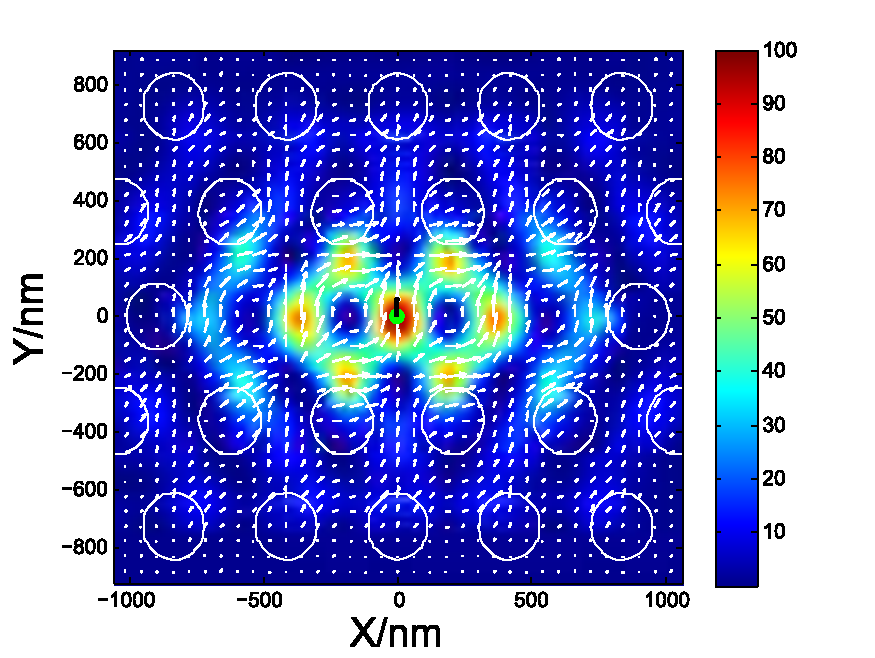
\includegraphics[width=1.1\textwidth]{./Figs/dotsmode1_1}
\end{center}
\caption[Dipole and E-field distributions in a H3 PC cavity structure.]{Dipole and E-field distribution in a H3 PC cavity structure.}
\label{dotsmode1_1}
\end{figure}

\column{0.5\textwidth}
\begin{figure}[htp]%[floatfix]
  \centering
 \begin{center}
 %\DeclareGraphicsRule{.pdf}{eps}{}{`convert #1 eps:-}
 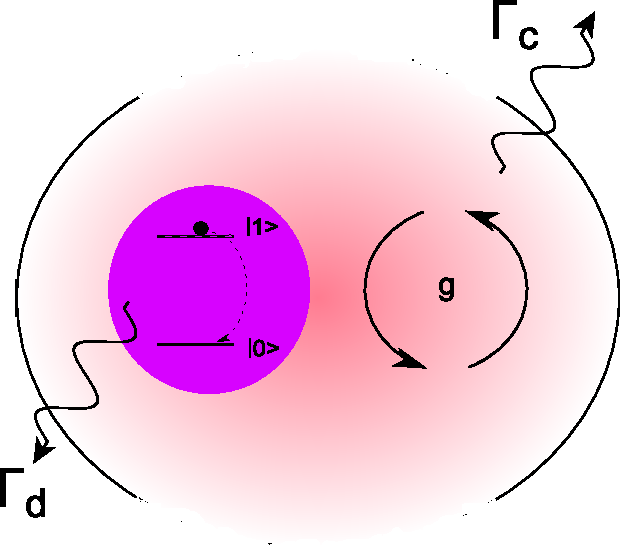
\includegraphics[width=0.7\textwidth]{./Figs/Cavity_withDipoleT}%[bb=1.0in 1.0in 7.5in 10in]
 \end{center}
 \caption[A diagram of a cavity with one dipole.]{A diagram of a cavity with one dipole. }
 \label{Cavity_withDipoleT}
 \end{figure}

\end{columns}
\end{frame}

\begin{frame}{One QD Coupled to A PC Cavity}
%\begin{columns}
%\column{0.5\textwidth}
\begin{figure}[H]
%\fontsize{18}{19}\selectfont
\centering
\begin{center}
%\psfrag{(w-w0)/meV}{$(\omega-\omega_c)/meV$}
%\psfrag{realG}{real$\bG$}
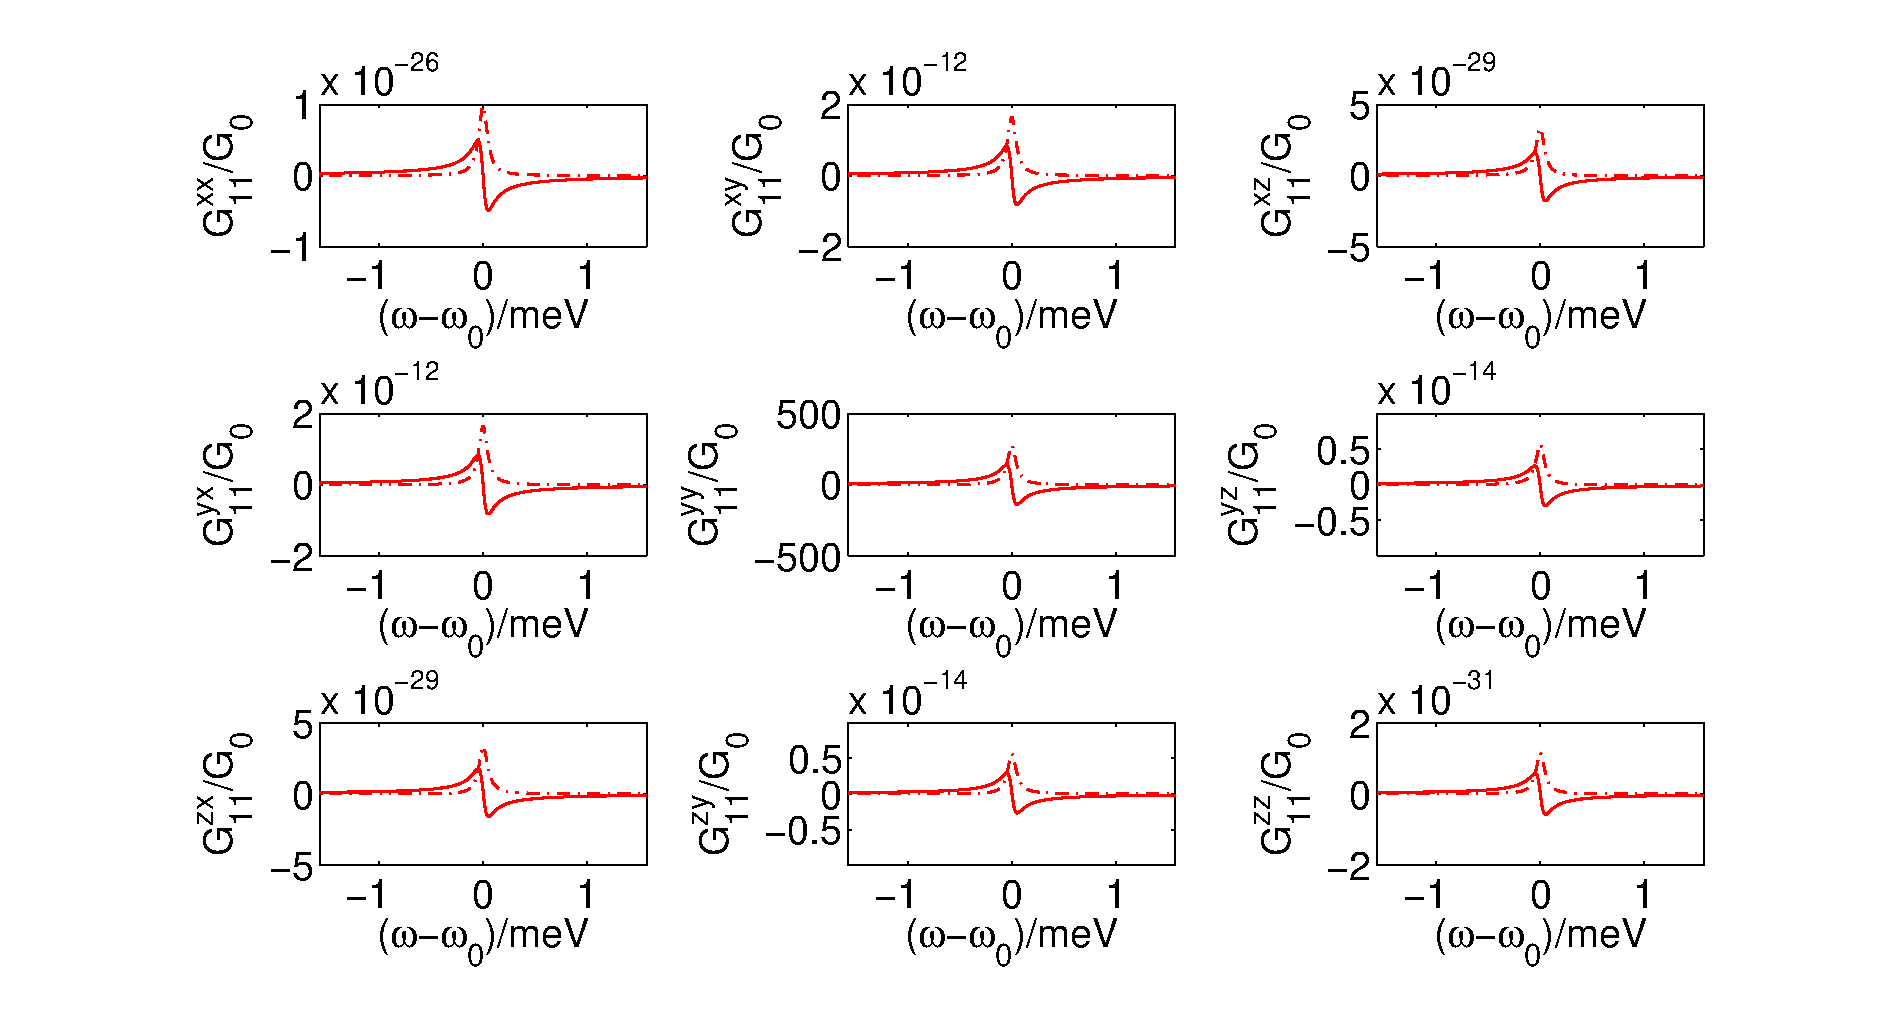
\includegraphics[width=0.95\textwidth]{./Figs/G84_11_1}
\end{center}
\caption[Diagram of GFT tensor elements.]{Full elements of $\mathbf{G}^0$ with $\omega_c/2\pi = 317 {\text {THz}}, \Gamma_c = 0.1 {\text {meV}}$.}
\label{G84_11_1}
%\normalsize
\end{figure}
\end{frame}


\begin{frame}{One QD Coupled to A PC Cavity}
%\column{0.5\textwidth}
\begin{figure}[H]
\centering
\begin{center}
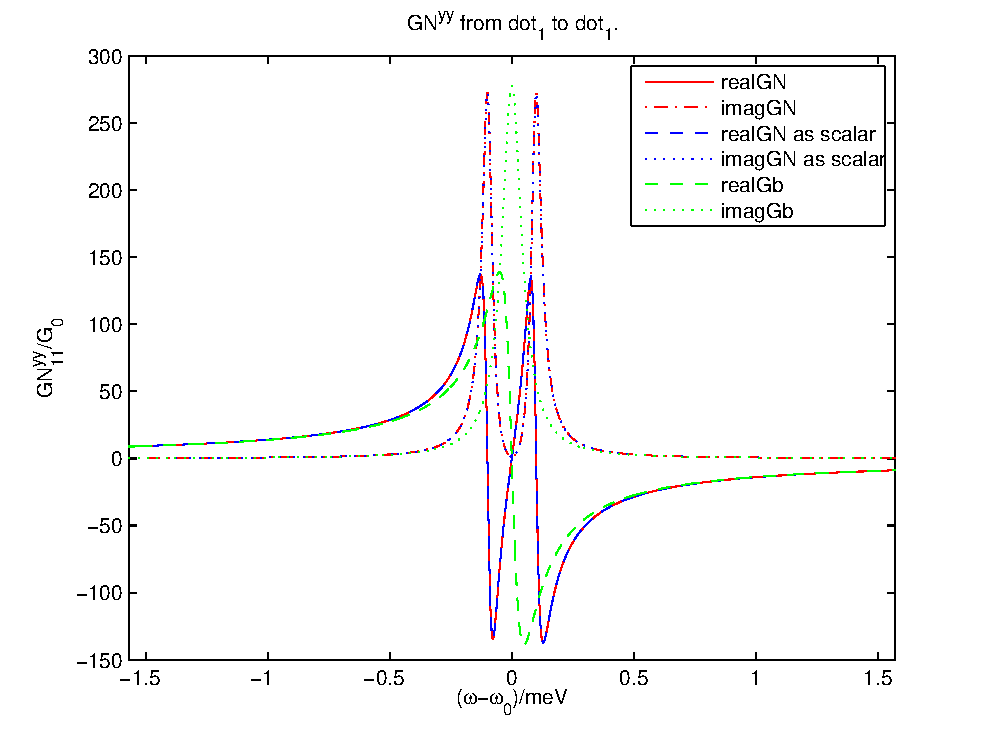
\includegraphics[width=0.7\textwidth]{./Figs/G84_yy11_1}
\end{center}
\caption[yy component of $G^1(\mathbf{r}_1,\mathbf{r}_1)$ with an on-resonance dipole.]{ yy component of $\mathbf{G}^1(\mathbf{r}_1,\mathbf{r}_1)$ with an on-resonance dipole of $\omega_d/2\pi = 317 {\text {THz}}, \Gamma_d = 2 \mu{\text {eV}}$.}
\label{G84_yy11_1}
\end{figure}
%\end{columns}
\end{frame}


\begin{frame}{Frequencies repulsion and splitting}
\begin{columns}
\column{0.5\textwidth}
\begin{figure}[H]
%\fontsize{18}{19}\selectfont
\centering
\begin{center}
%\psfrag{(w-w0)/meV}{$(\omega-\omega_c)/meV$}
%\psfrag{realG}{real$\bG$}
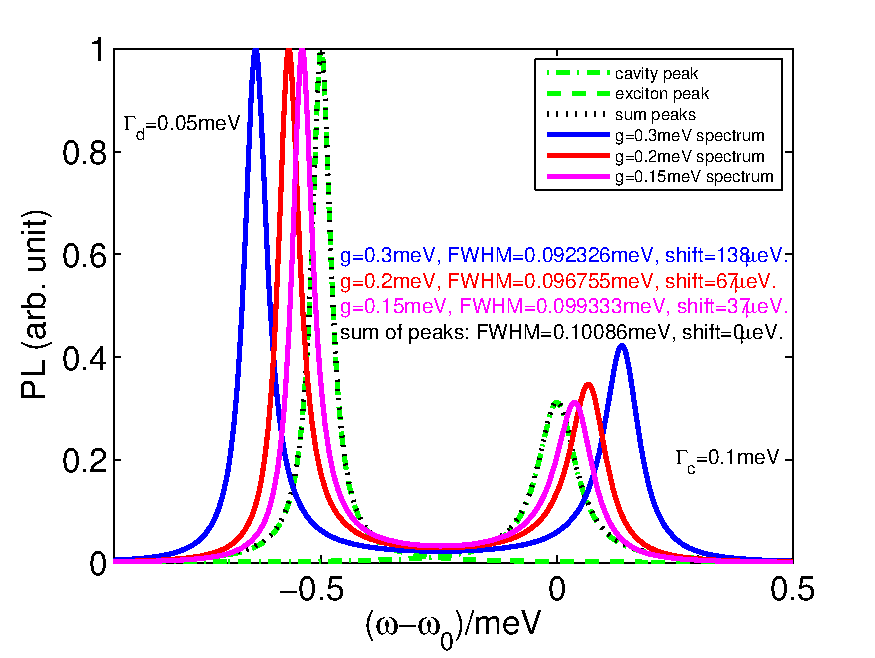
\includegraphics[width=1.1\textwidth]{./Figs/gincreased1}
\end{center}
\caption[Spec of off-resonance cavity.]{Off-resonance case with increasing $ g $.}
\label{gincrease1}
%\normalsize
\end{figure}

\column{0.5\textwidth}
\begin{figure}[H]
\centering
\begin{center}
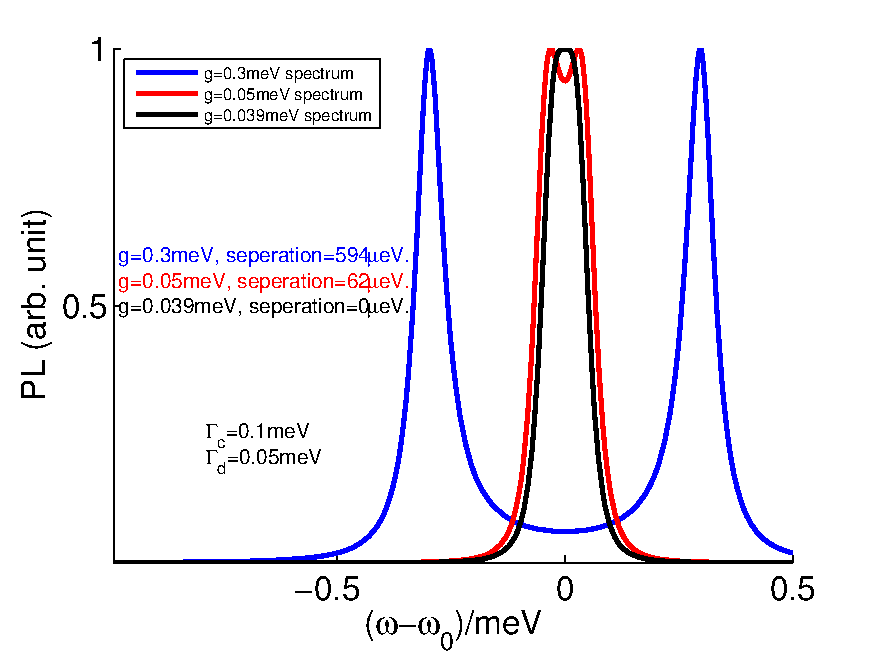
\includegraphics[width=1.1\textwidth]{./Figs/gincreased_onresonance}
\end{center}
\caption[Spec with an on-resonance dipole.]{On-resonance case with increasing $ g $.}
\label{gincrease2}
\end{figure}
\end{columns}
\end{frame}

\begin{frame}{A Cavity Coupled to Many Excitons}
\begin{figure}[htp]%[floatfix]
\centering
\begin{center}
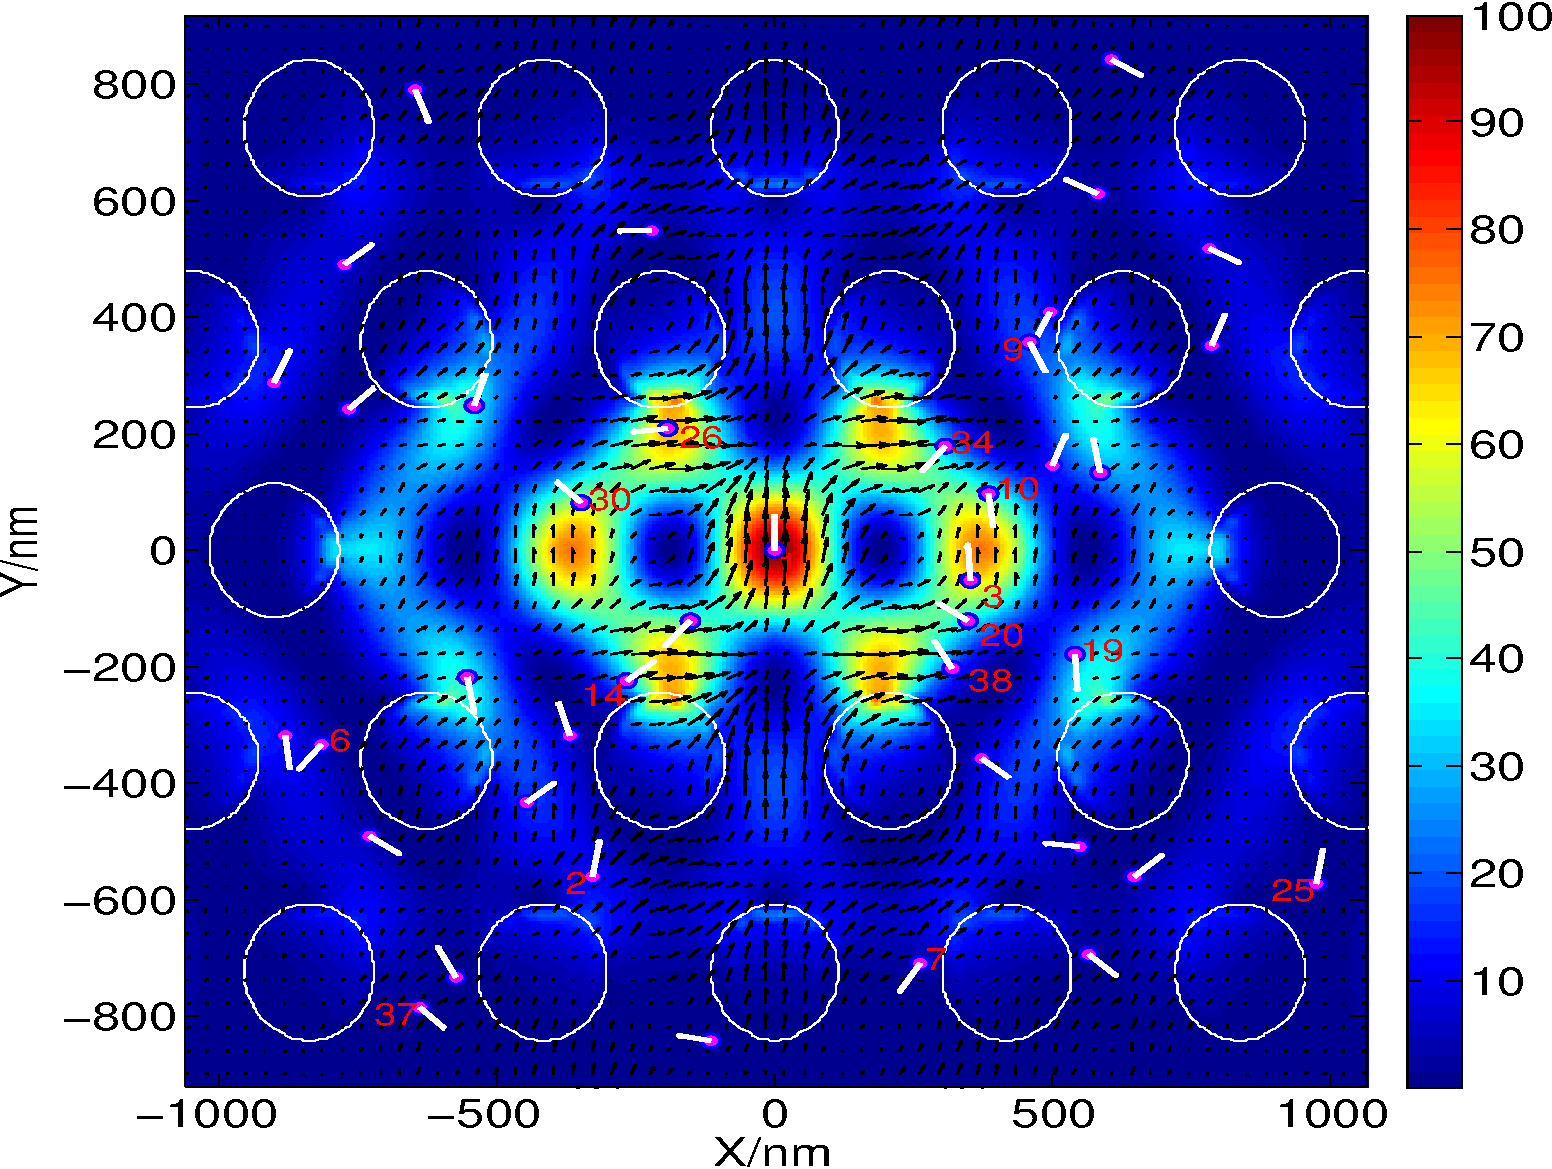
\includegraphics[width=0.7\textwidth]{./Figs/QDmode}
\end{center}
\caption[Cavity mode and 41-QD distribution in a PC cavity.]{Cavity mode and QDs distributions map. }
\label{QDmode}
\end{figure}
\end{frame}

\begin{frame}{A Cavity Coupled to Many Excitons}
\begin{columns}
\column{0.6\textwidth}
\begin{figure}[htp]%[floatfix]
\centering
\begin{center}
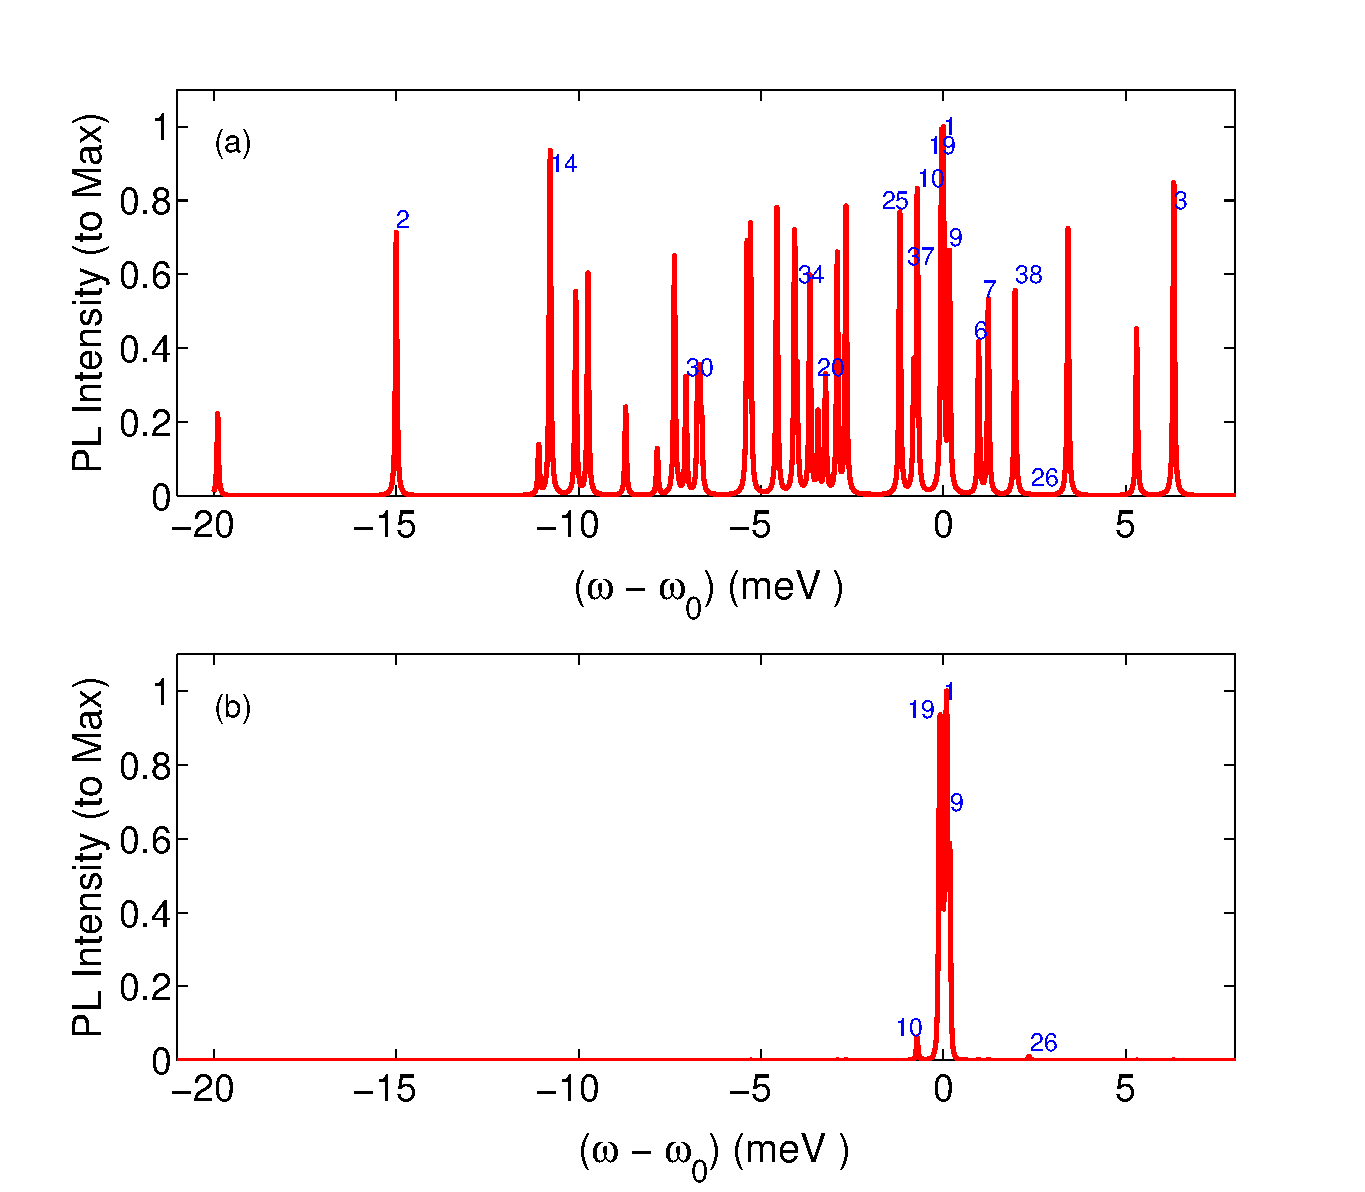
\includegraphics[width=0.8\textwidth]{./Figs/QDspecPChom}
\end{center}
\caption[Spectra of 41 QDs in a homogeneous medium and a PC cavity.]{\fontsize{8}{-0.2}\selectfont $Y$-polarized Spectra of 41 QDs in a homogeneous medium (a) and the PC cavity (b). The QDs ensemble has a Gaussian distribution profile, centered at 5 meV lower than the cavity mode resonance, with standard deviation $\sigma=20$ meV.}
\label{QDspecPChom}
\end{figure}

\column{0.4\textwidth}
\begin{figure}[htp]%[floatfix]
\centering
\begin{center}
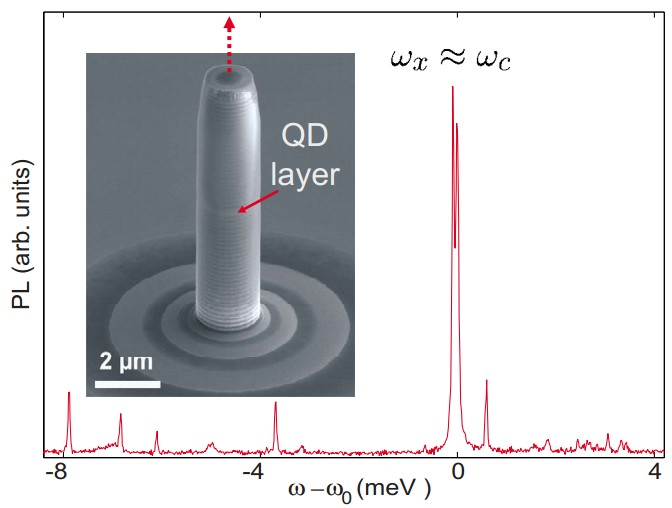
\includegraphics[width=0.99\textwidth]{./Figs/ExperimentalSpec}
\end{center}
\caption[Spectra of a PC cavity in experiment.]{\fontsize{8}{-0.2}\selectfont Experimental spectrum of an optical cavity coupled to excitons. Adapted from P. Yao, P. Pathak, etc. \textit{PRB}, \textbf{2010}, \textit{81}, 33309. 
}
\label{specexp1}
\end{figure}

\end{columns}
\end{frame}

\subsection{Pump Dynamics}

\begin{frame}{Collective Emission Under Optical Pump}
\begin{columns}
\column{0.4\textwidth}
\begin{figure}[htp]%[floatfix]
\centering
\begin{center}
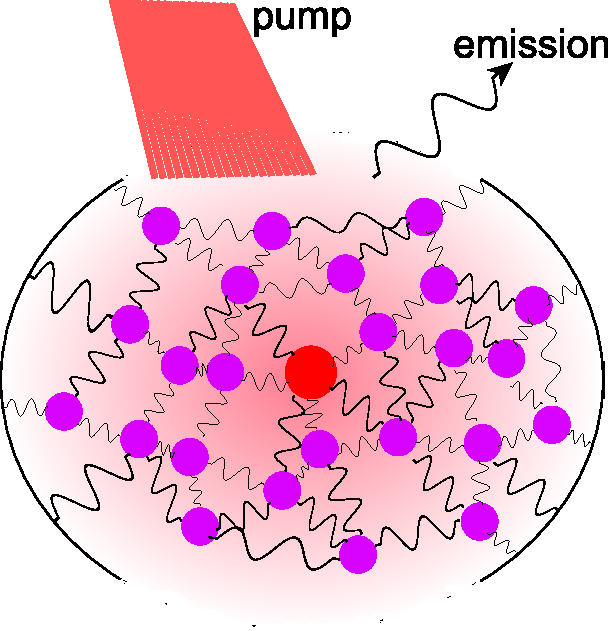
\includegraphics[width=0.8\textwidth]{./Figs/Cavity_pump}
\end{center}
\caption[Pumping a cavity.]{\fontsize{8}{-0.2}\selectfont A cavity under pumping.}
\label{pumpcavity}
\end{figure}

\column{0.6\textwidth}
\fontsize{8}{-0.2}\selectfont 
Master equation for one exciton coupled cavity:
\begin{equation}
\begin{split}
  \dt \rho & = \frac{1}{i\hbar}[H_s,\rho]\! +\! \frac{\Gamma_c+P_c}{2}(2a\rho\adag\! -\! \adag a\rho\! -\! \rho\adag a)\\
& +\frac{\Gamma_x+P_x}{2}(2\sigm\rho\sigp - \sigp\sigm\rho - \rho\sigp\sigm ) \\
& +\frac{P_c}{2}(2\adag\rho a - a \adag\rho - \rho a\adag) \\
&+ \frac{P_x}{2} (2\sigp\rho\sigm - \sigm\sigp\rho - \rho\sigm\sigp )\\
&+\frac{\Gamma_x^{\prime}}{4} (\sigz\rho\sigz-\rho),\nonumber
 \end{split}
\end{equation}
where the system Hamiltonian under the rotating wave approximation is given by
\begin{equation}
 H_s=\hbar\omega_c \adag a+ \hbar \Omega_x \sigp\sigm +\hbar g(\sigm \adag+\sigp a).\nonumber
\end{equation}
\end{columns}

\end{frame}



\begin{frame}{Collective Emission Under Optical Pump}

\begin{figure}[h]%[floatfix]
     \centering
     \subfigure{
          %\label{fig:GFT_ME_spec_str}
          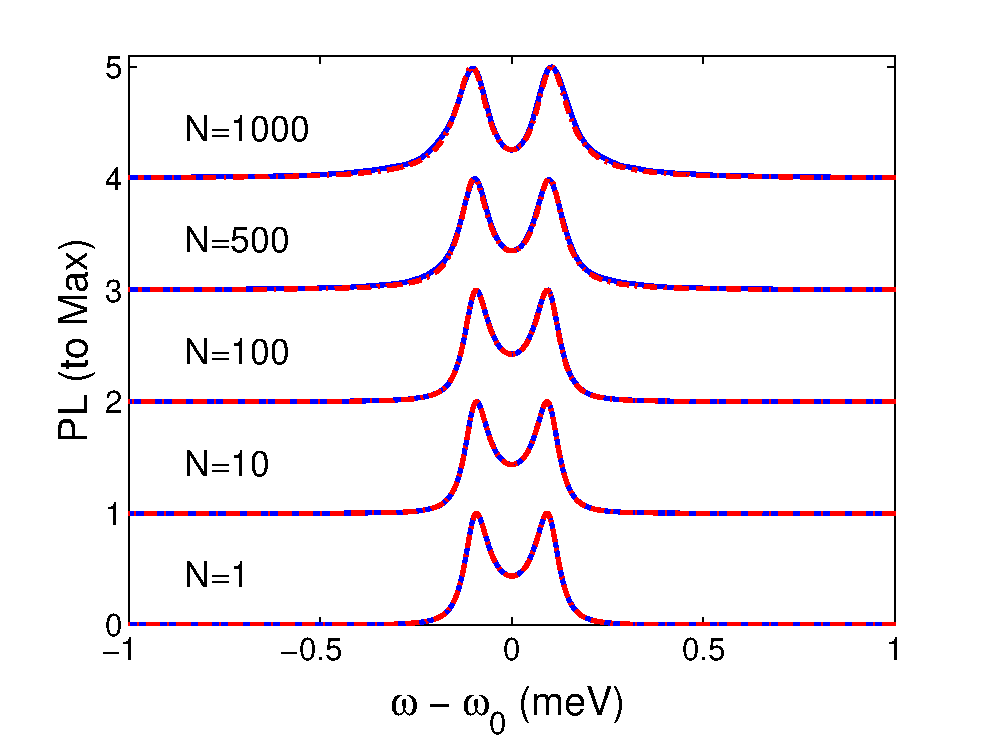
\includegraphics[width=.46\textwidth]{./Figs/GFT_ME_spec_str}}
     \subfigure{
          %\label{fig:P_str}
          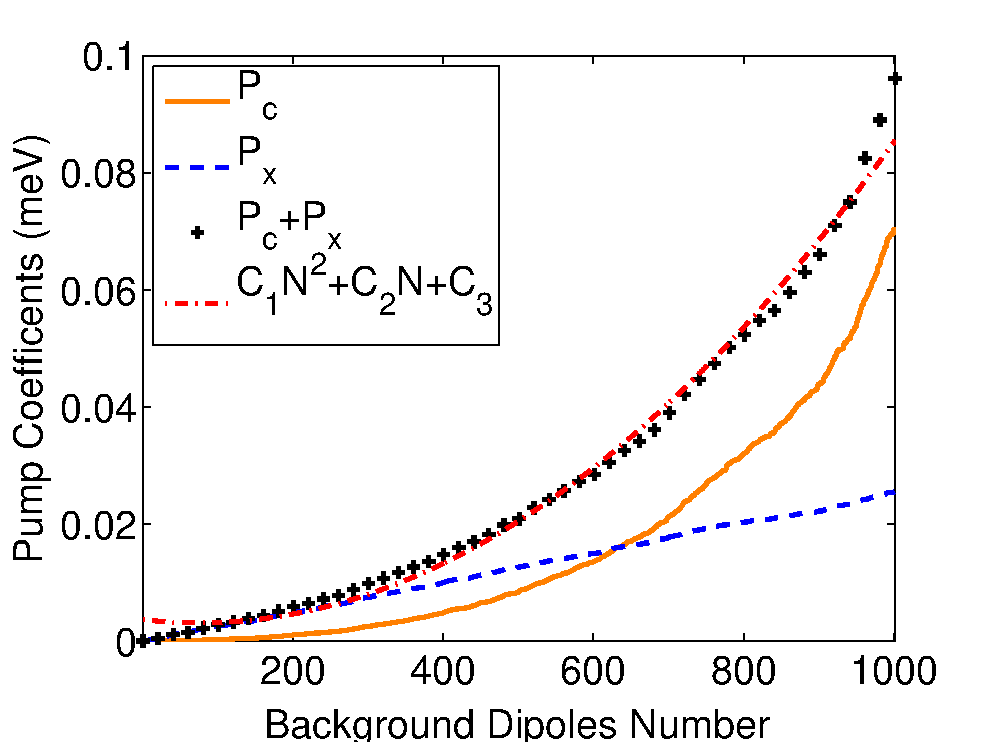
\includegraphics[width=.46\textwidth]{./Figs/P_str}}
     \caption[Pumping as a tool for dipoles excitation.]{ \fontsize{8}{0.2}\selectfont
       Least Square fit of ME model to GFT spectra as background dipoles number $N$ varies from $0$ to $1000$. Target exciton is on-resonance.  The GFT spectra (solid-blue curves left) are averaged of $400$ samples, each of which has up to $1000$ background dipoles Gaussianly distributed around the cavity resonance with a standard deviation of $\sigma=20$ meV. The best fit ME pumping coefficients $P_c+P_x$ show a good function form of $C_1N^2+C_2N+C_3$.
       }
     %\label{fig:GFT_ME_fits1}
 \end{figure}
\end{frame}




\begin{frame}{Collective Emission Under Optical Pump}

\begin{figure}[htp]%[floatfix]
     \centering
      \subfigure{
           %\label{fig:GFT_ME_spec_weak}
           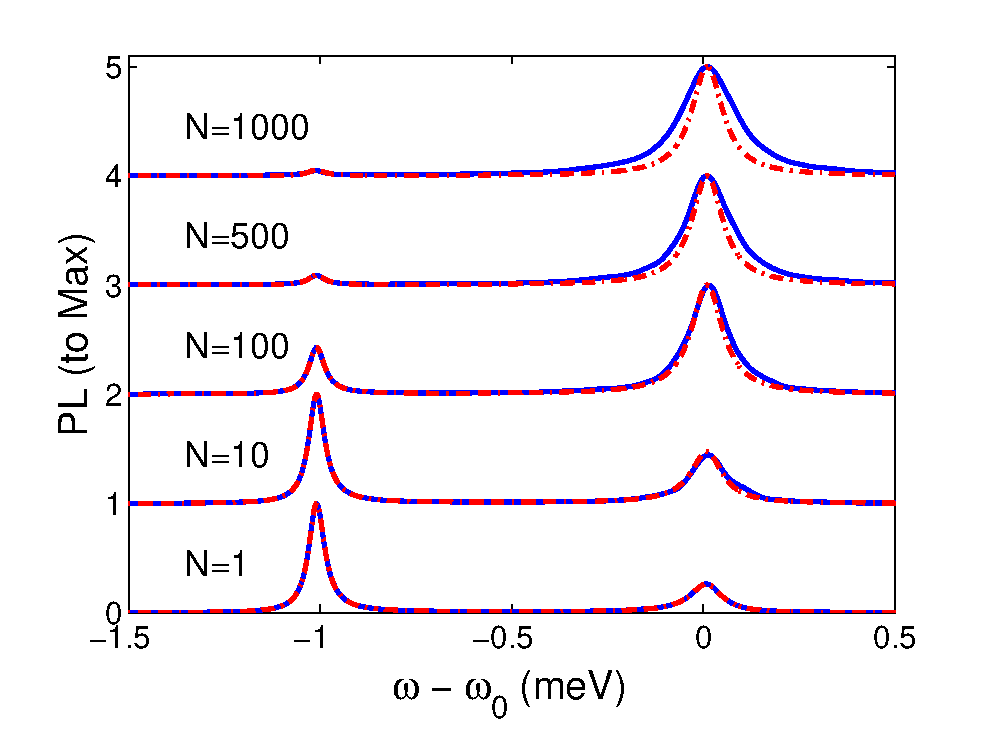
\includegraphics[width=.46\textwidth]
                {./Figs/GFT_ME_spec_weak}}
     \subfigure{
           %\label{fig:P_weak}
          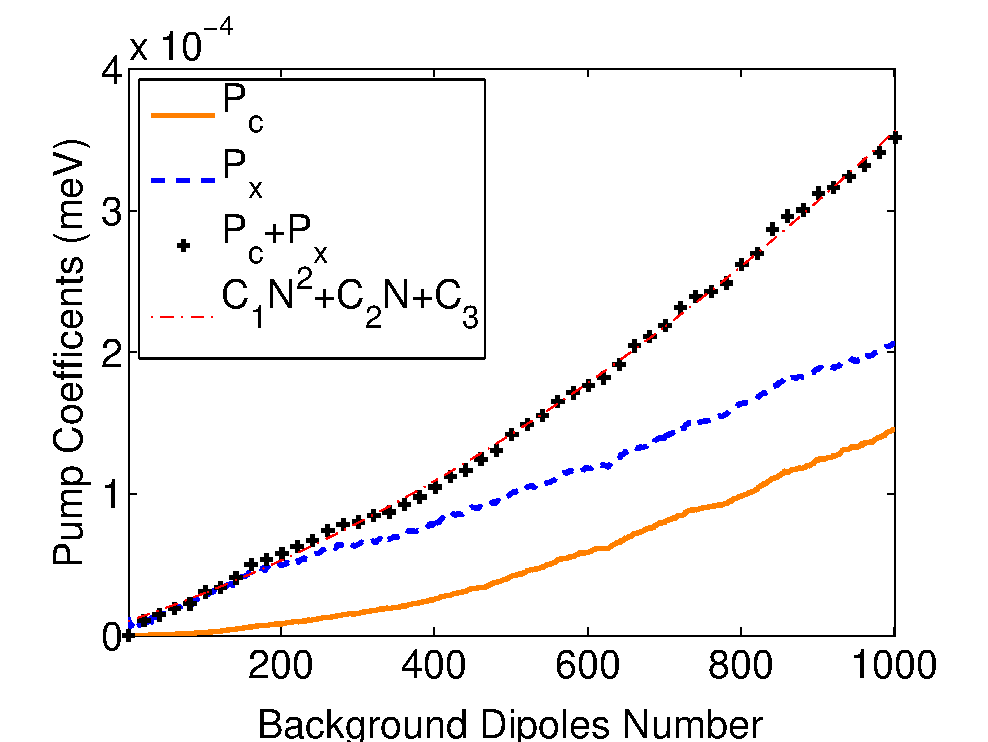
\includegraphics[width=.46\textwidth]{./Figs/P_weak}}
       \caption[Pumping as a tool for dipoles excitation.]{ \fontsize{8}{0.2}\selectfont
       Least Square fit of ME model to GFT spectra as background dipoles number $N$ varies from $0$ to $1000$. The target exciton is off-resonance. The GFT spectra (solid-blue curves left) are averaged of $400$ samples, each of which has up to $1000$ background dipoles Gaussianly distributed around the cavity resonance with a standard deviation of $\sigma=20$ meV. The best fit ME pumping coefficients $P_c+P_x$ show a good function form of $C_1N^2+C_2N+C_3$.
       }
    %\label{fig:GFT_ME_fits2}
   \end{figure}
\end{frame}

\begin{frame}{Interpretations of Pumping Dynamics}
\begin{figure}[htp]%[floatfix]
\centering
\begin{center}
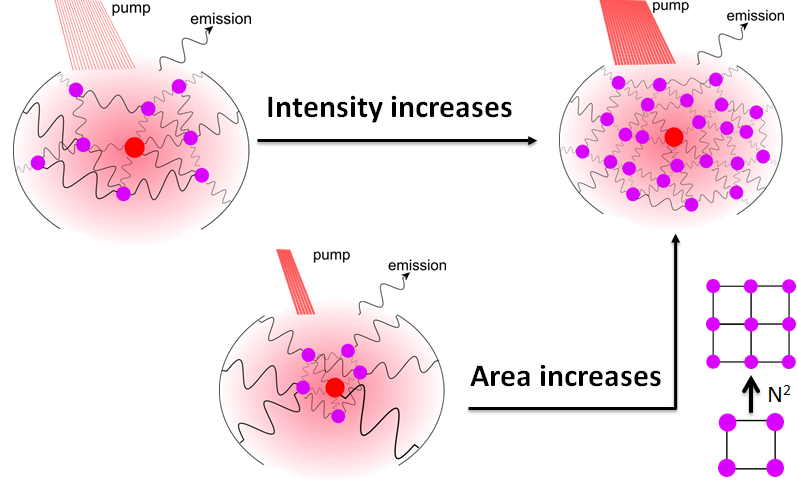
\includegraphics[width=0.8\textwidth]{./Figs/pumpingdynamics}
\end{center}
\caption[Pumping a cavity.]{\fontsize{8}{-0.2}\selectfont Interpretations of pumping dynamics.}
\label{pumpdyn}
\end{figure}
\end{frame}

\subsection[Resonance Shifting and spectral broadening effects]{Resonance Shifting and spectral broadening effects of Dense-exciton Coupled Cavities}
\begin{frame}{Fully Off-resonance Case}
\begin{columns}
\column{0.5\textwidth}
\begin{figure}[htp]%[floatfix]
\centering
\begin{center}
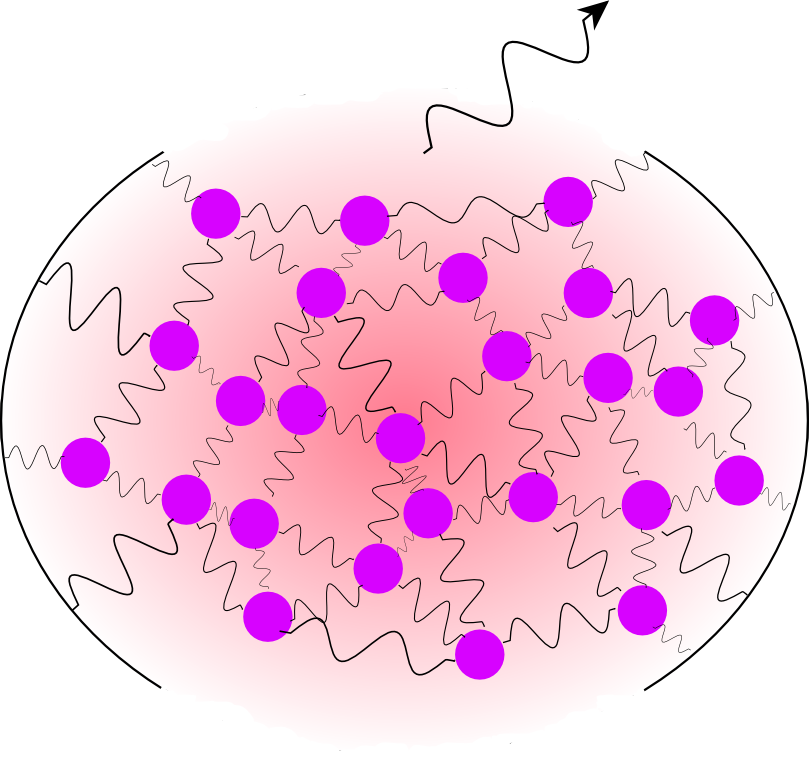
\includegraphics[width=0.8\textwidth]{./Figs/Cavity_manyBackgroundDipoles}
\end{center}
\caption[off-resonance case.]{\fontsize{8}{-0.2}\selectfont A cavity with off-resonance excitons.}
\label{offresonance}
\end{figure}

\column{0.5\textwidth}
\begin{figure}[htp]%[floatfix]
\centering
\begin{center}
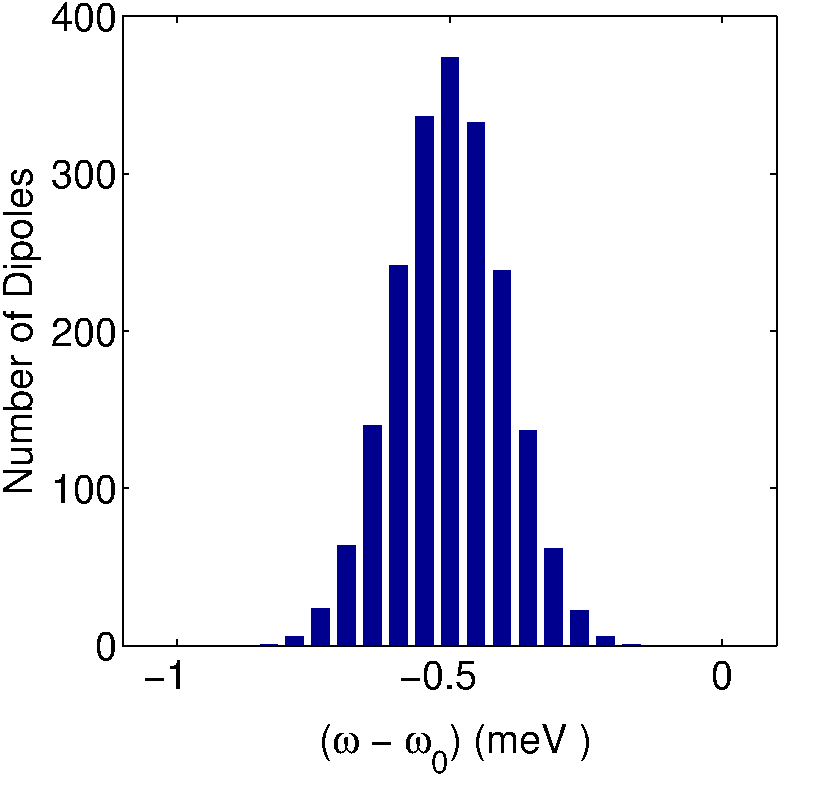
\includegraphics[width=0.8\textwidth]{./Figs/distr_wd0dot5s0dot1}
\end{center}
\caption[off-resonance case.]{\fontsize{8}{-0.2}\selectfont Resonance distribution of excitons with $\sigma=0.1$ meV and $\Delta\omega=-0.5$ meV.}
\label{distr_offresonance1}
\end{figure}
\end{columns}
\end{frame}

\begin{frame}{Fully Off-resonance Case}
\fontsize{8}{-0.2}\selectfont
The Green functions including $n$-dipoles (labeled by $(n)$ in the superscripts) are
\begin{align}
\label{Gn11}
 G^{(n)}_{R_b,R_b}&=\frac{G^{(0)}_{R_b,R_b}}{1-G^{(0)}_{R_b,R_b}\sum_i^n{\alpha_i}},\\
\label{GnR1}
 G^{(n)}_{R,R_b}&=\frac{G^{(0)}_{R,R_b}}{1-G^{(0)}_{R_b,R_b}\sum_j^n{\alpha_j}}.
\end{align}
For short hand, we have labeled the first subscript of GFs as the detector,
and labeled the second subscript of GFs as the source.
\vskip10pt
Particularly, if all background dipoles share the same resonance and optical moment, it leads to
\begin{equation}
\sum_j^n{\alpha_j}=n\alpha,
\end{equation}
which means that, if we treat the ensemble as a single dipole, the effective optical moment and effective coupling strength are enlarged by $\sqrt{N}$ folds from the individual dipole. 
\end{frame}

\begin{frame}{Fully Off-resonance Case}
\begin{columns}
\column{0.5\textwidth}
\begin{figure}[htp]%[floatfix]
\centering
\begin{center}
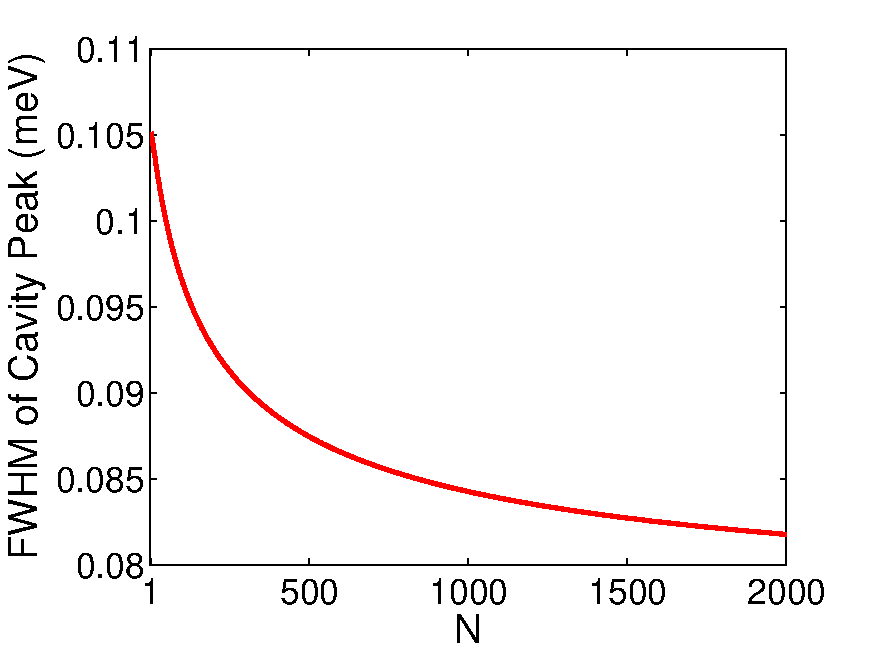
\includegraphics[width=0.8\textwidth]{./Figs/FWHMcav_2000wd0dot5s0dot1}
\end{center}
\caption[off-resonance case.]{\fontsize{8}{-0.2}\selectfont FWHM of A cavity with off-resonance excitons.}
\label{offresonance_FWHM}
\end{figure}

\column{0.5\textwidth}
\begin{figure}[htp]%[floatfix]
\centering
\begin{center}
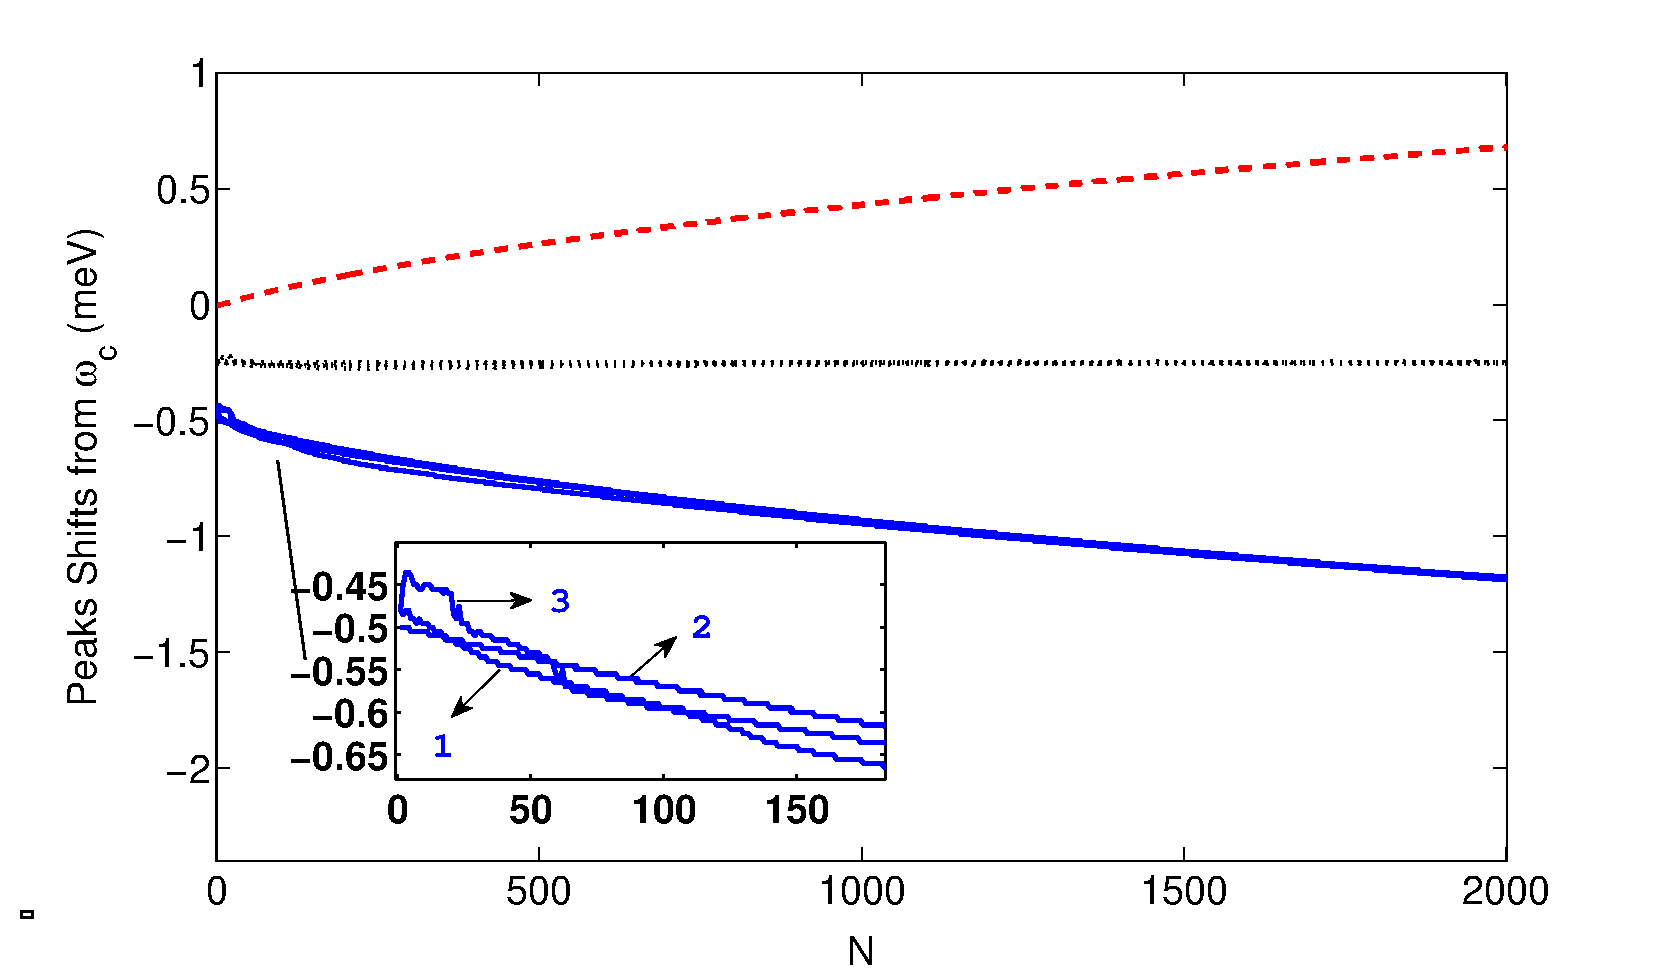
\includegraphics[width=1.09\textwidth]{./Figs/peakshift_wd0dot5_detune_N}
\end{center}
\caption[off-resonance case.]{\fontsize{8}{-0.2}\selectfont Cavity resonance shift as $ N $ increases. Inset is a magnified segment of dipole peak position,
where label 1 corresponds to the single-dipole case and equivalent to the $\sigma=0$ case,
label 2 shows the $\sigma=0.05$ meV case,
and label 3 shows the $\sigma=0.1$ meV case.
The difference between the curves is small.}
\label{offresonance1}
\end{figure}
\end{columns}
\end{frame}



\begin{frame}{With an on-resonance target dipole}
\begin{columns}
\column{0.5\textwidth}
\begin{figure}[htp]%[floatfix]
\centering
\begin{center}
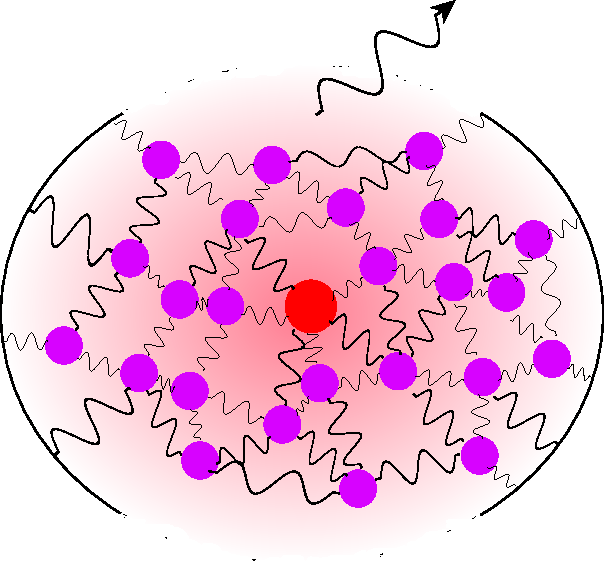
\includegraphics[width=0.8\textwidth]{./Figs/Cavity_withTargetDipole}
\end{center}
\caption[off-resonance case with a target dipole.]{\fontsize{8}{-0.2}\selectfont A cavity coupled to a background exciton ensemble and a target exciton.}
%\label{offresonance}
\end{figure}

\column{0.5\textwidth}
\begin{figure}[htp]%[floatfix]
\centering
\begin{center}
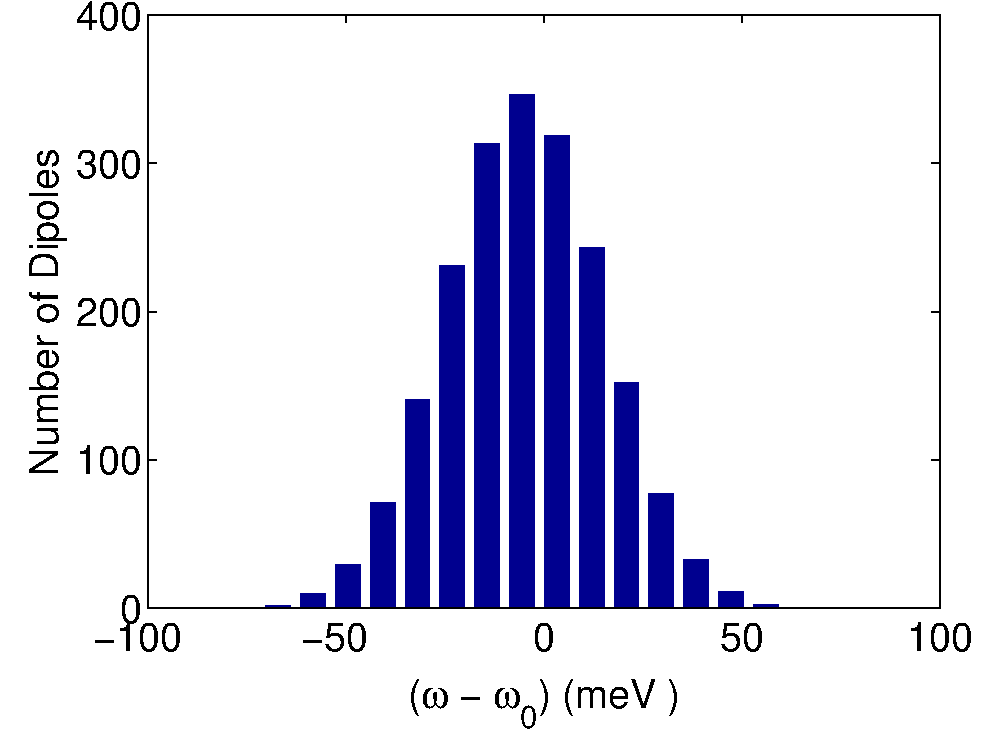
\includegraphics[width=0.9\textwidth]{./Figs/wddistr_wdrand5s20_qd2000_stat200}
\end{center}
\caption[Background exciton distribution.]{\fontsize{8}{-0.2}\selectfont The Gaussian distribution profile of dipole resonances with $\sigma=20$ meV and $\Delta\omega=-5$ meV.}
\label{offresonance_distr2}
\end{figure}
\end{columns}
\end{frame}


\begin{frame}{With an on-resonance target dipole}
\fontsize{8}{0.2}\selectfont

\begin{columns}
\column{0.5\textwidth}
If there is one target dipole with a relatively large coupling strength and all the other background dipoles are in a mean weak field, the GFs are
\begin{subequations}
%\label{G1RR}
\begin{align}
 G^{(1)}_{R_t,R_j} &=\frac{G^{(0)}_{R_t,R_j}}{1-G^{(0)}_{R_t,R_t}\alpha_t},\quad j=t,b,\nonumber\\
  G^{(1)}_{R,R_t} &=\frac{G^{(0)}_{R,R_t}}{1-G^{(0)}_{R_t,R_t}\alpha_t}, \nonumber\\
  G^{(1)}_{R,R_b} &=G^{(0)}_{R,R_b}+\frac{G^{(0)}_{R,R_t}\alpha_t G^{(0)}_{R_t,R_b}}{1-G^{(0)}_{R_t,R_t}
  \alpha_t},\nonumber\\
  G^{(1)}_{R_b,R_b} &=G^{(0)}_{R_b,R_b}+\frac{G^{(0)}_{R_b,R_t}\alpha_t G^{(0)}_{R_t,R_b}}{1-G^{(0)}_{R_t,R_t}\alpha_t},\nonumber
  %\label{G1RbRb}
\end{align}
\end{subequations}

\column{0.5\textwidth}
and for $n\geq 1$
%\begin{subequations}
%\label{Gn+1RtRj}
\begin{align}
 G^{(n+1)}_{R_t,R_j} 
% &=\frac{G^{(n)}_{R_t,R_j}}{1-G^{(n)}_{R_t,R_t}\alpha_t} \nonumber\\
 %\label{Gn+1RtRj1}\\
&= \frac{G^{(1)}_{R_t,R_j}}{1-G^{(1)}_{R_b,R_b}\sum_p^n{\alpha_p}},\quad j=b,t,\nonumber
%\label{Gn+1RtRjexpand}
\end{align}
%\end{subequations}
\begin{align}
  G^{(n+1)}_{R,R_b} &=\frac{G^{(1)}_{R,R_b}}{1-G^{(1)}_{R_b,R_b}\sum_i^n{\alpha_i}},\nonumber \\
 G^{(n+1)}_{R,R_t} &=G^{(n)}_{R,R_t}+\frac{G^{(n)}_{R,R_b}\alpha_n G^{(n)}_{R_b,R_t}}{1-G^{(n)}_{R_b,R_b}\alpha_n},\nonumber \\
 %\label{Gn+1RRt}\\
  G^{(n+1)}_{R_b,R_b} &=\frac{G^{(1)}_{R_b,R_b}}{1-G^{(1)}_{R_b,R_b}\sum_i^n{\alpha_i}}.\nonumber
  %\label{Gn+1RbRb}
\end{align}
\end{columns}
\end{frame}


\begin{frame}{Case 1: $ g_t=g_b=g=0.02 $meV, $ \Delta \omega=-5 $meV.}
\begin{figure}[htp]%[floatfix]
\centering
\begin{center}
%\psfrag{PL}{$PL (to Max)$}
%\psfrag{omega-omega}{$\omega-\omega_c (meV)$}
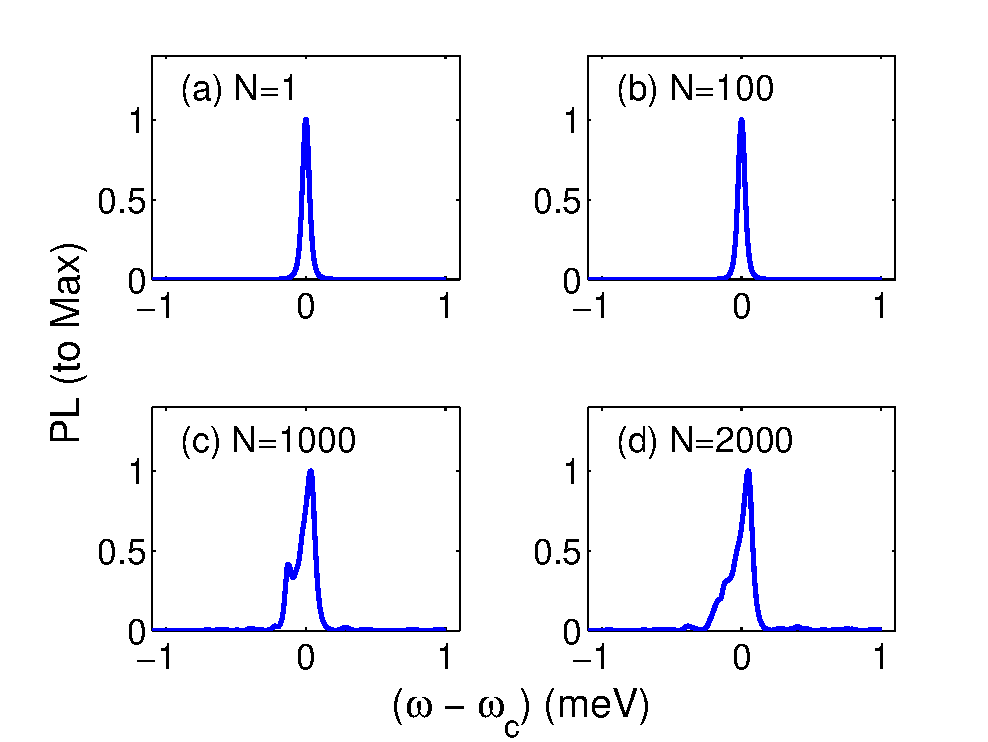
\includegraphics[width=0.8\textwidth]{./Figs/spec_wdrand5s20_E0dot2_qd2000_stat200_sam1} %spec_wdrand5s20_E0.2_qd2000_stat200_sam32.eps
\end{center}
\caption[Spectra samples for $N$ background excitons coupled cavity]{  Cavity spectra of one set of exciton samples with various background exciton populations $N$. We used $\Delta\omega=-5$ meV and $\sigma=20$ meV.}
%\label{spec_wdrand5s20_E0.2_qd2000_stat200_sam32}
\end{figure}

\end{frame}



\begin{frame}{Case 1: $ g_t=g_b=g$.}
\begin{figure}[htp]%[floatfix]
\centering
\begin{center}
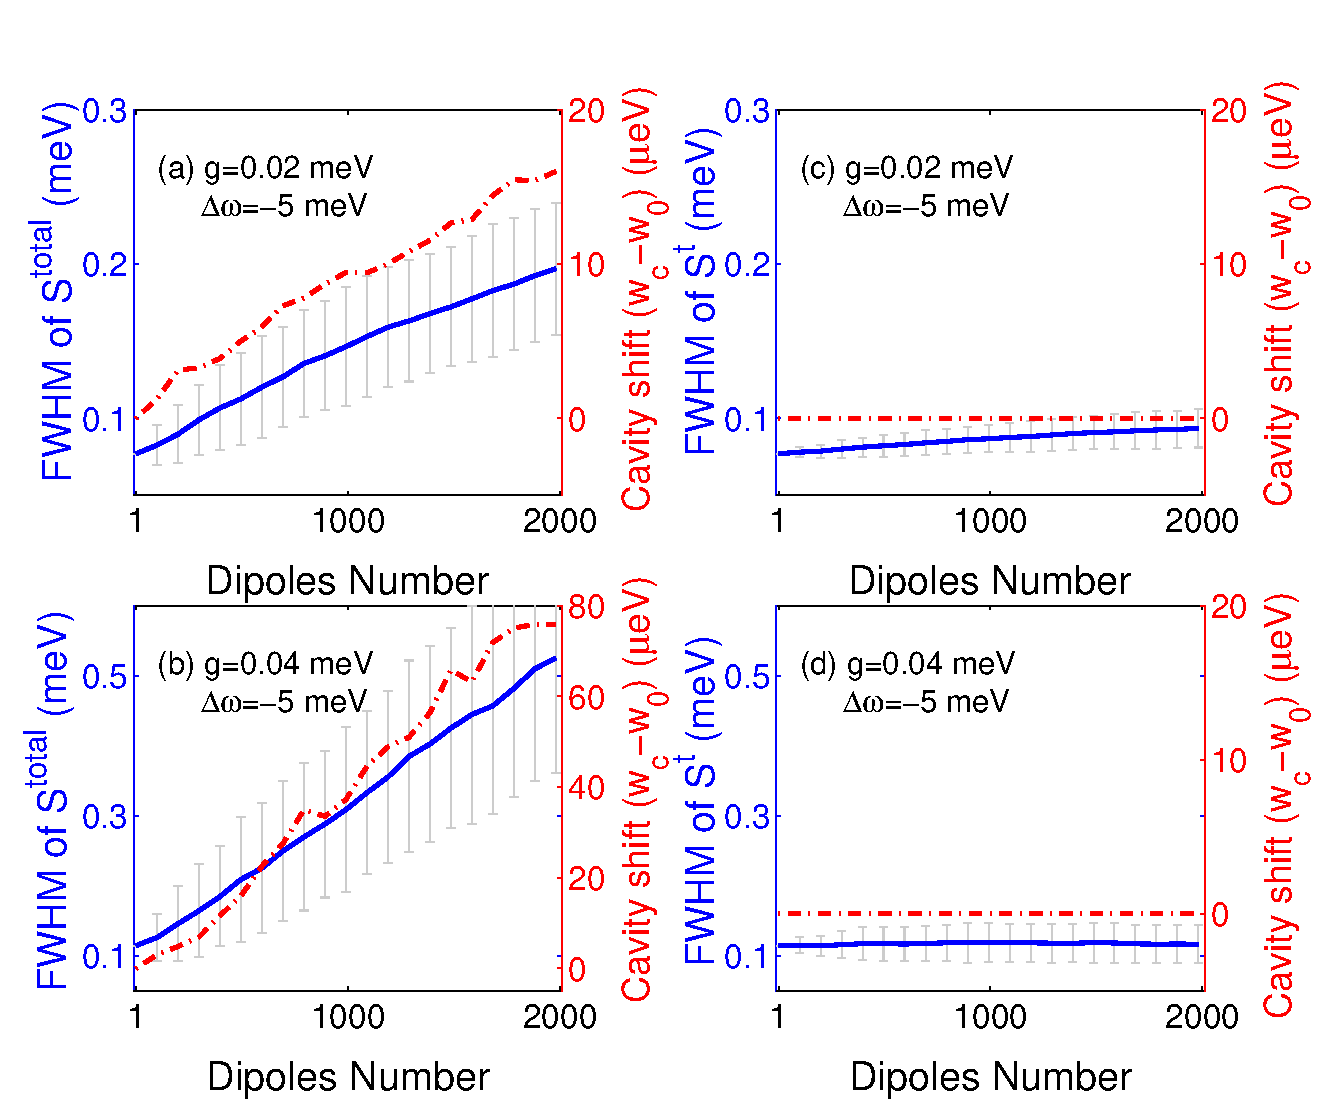
\includegraphics[width=0.74\textwidth]{./Figs/fwhm_wdrand5s20_E0dot2-0dot4_qd2000_stat200}
\end{center}
\caption[Spectral modification by pure background dipoles.]{ FWHMs (blue solid line) and peaks shifts (red dashed line) of cavity and dipole 1 spectra with a dipoles ensemble of the same coupling strength $g$. Curves are averaged over 200 samples with the same distribution function. The gray vertical bars around blue line demonstrate the standard deviation of the FWHM obtained from 200 statistical samples. The cavity resonance shift is referenced to the bare cavity resonance with a high frequency shift as positive shift. (a) and (c) show the FWHM and peak shifts of the total cavity and QD 1 spectra respectively, with $g=0.02$ meV; (b) and (d) are with $g=0.04$ meV. Other parameters used are: $\Gamma_c=0.1$ meV, $\Gamma_d=0.05$ meV, bare cavity resonance $\omega_c=792.25$ meV, central angular frequency shift of dipoles ensemble $\Delta\omega=-5$ meV. }
\label{fwhm_wdrand5s20_E0.2-0.4_qd2000_stat200}
\end{figure}

\end{frame}



\begin{frame}{Case 2: $ g_t>g_b $, $ \Delta\omega=-5 $meV.}
\begin{figure}[H]%[floatfix]
\centering
\begin{center}
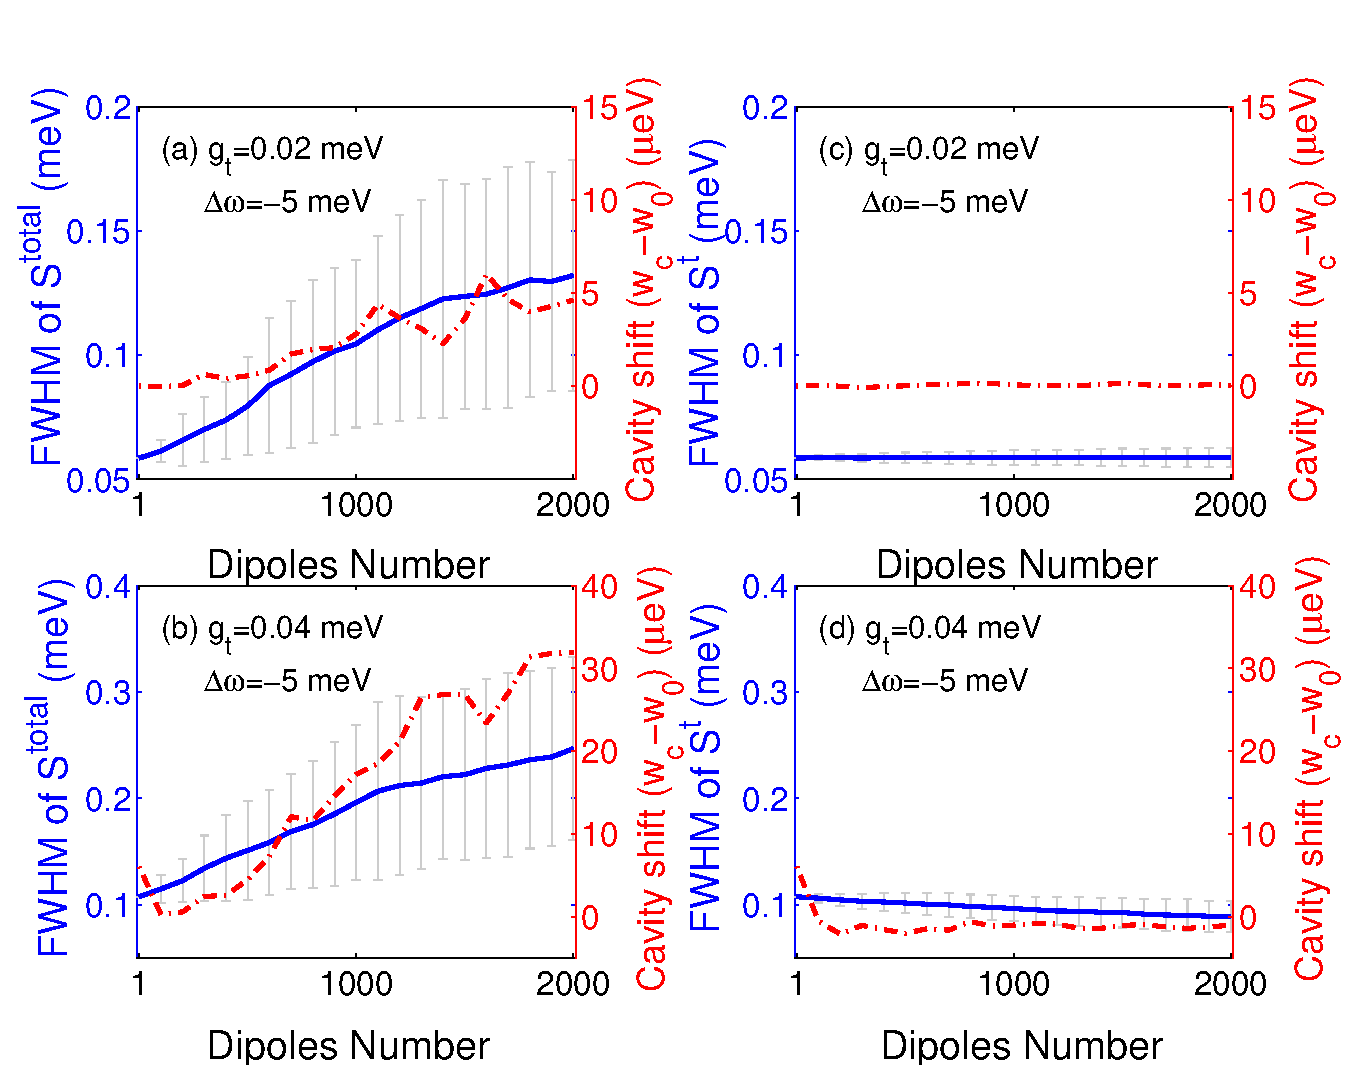
\includegraphics[width=0.78\textwidth]{./Figs/fwhm_wdrand5s20_gt0dot2-0dot4_qd2000_stat200}
\end{center}
\caption[Spectral modification of a cavity with a target dipole and an ensemble.]{  FWHMs (blue solid line) and peak cavity resonance shifts (red dashed line) of cavity mode spectrum for dipole ensemble with $g_b=0.5g_t$. All curves are averaged over 200 samples randomly generated under the same distribution function. The vertical gray bars around the blue line illustrates the standard deviation of the FWHM obtained from the 200 statistical samples. The cavity resonance shift is referenced to the bare cavity resonance with high frequency shift as positive shift. (a) and (c) show the respective total and target dipole spectral FWHMs and peak shifts with $g_t=0.02$ meV; (b) and (d) are for $g_t=0.04$ meV. Other parameters used to generate this graph were: $\Gamma_c=0.1$ meV, $\Gamma_{d}=0.05$ meV, bare cavity resonance $\omega_c=792.25$ meV, central angular frequency shift of dipoles ensemble $\Delta\omega=-5$ meV. }
\label{fwhm_wdrand5s20_gt0.2-0.4_qd2000_stat200}
\end{figure}
\end{frame}


\begin{frame}{Case 2: $ g_t=2g_b=0.02 $meV, changing $ \Delta\omega $.}
\begin{figure}[htp]
\centering
\begin{tabular}{cc}
  \subfigure[ ]{
    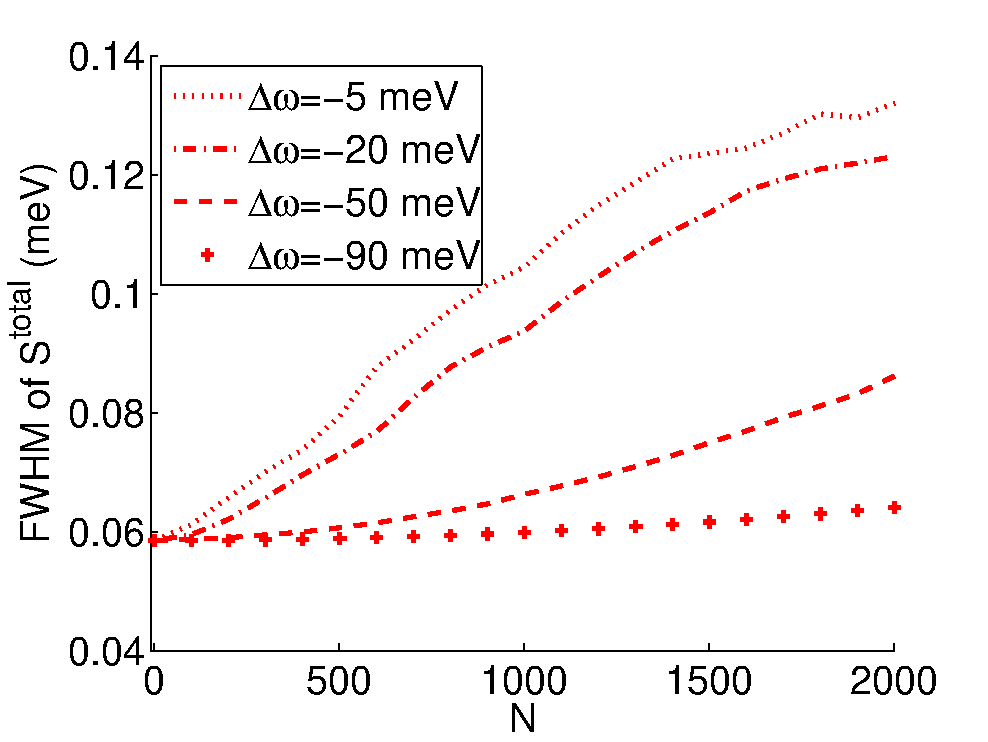
\includegraphics[width=0.33\textwidth]{./Figs/Stotalfwhm_wdrand5-90s20_gt0dot02b0dot5_qd2000_stat200}
    \label{Stotalfwhm_wdrand5-90s20_gt0.02b0.5_qd2000_stat200}}
 &
  \subfigure[ ]{
    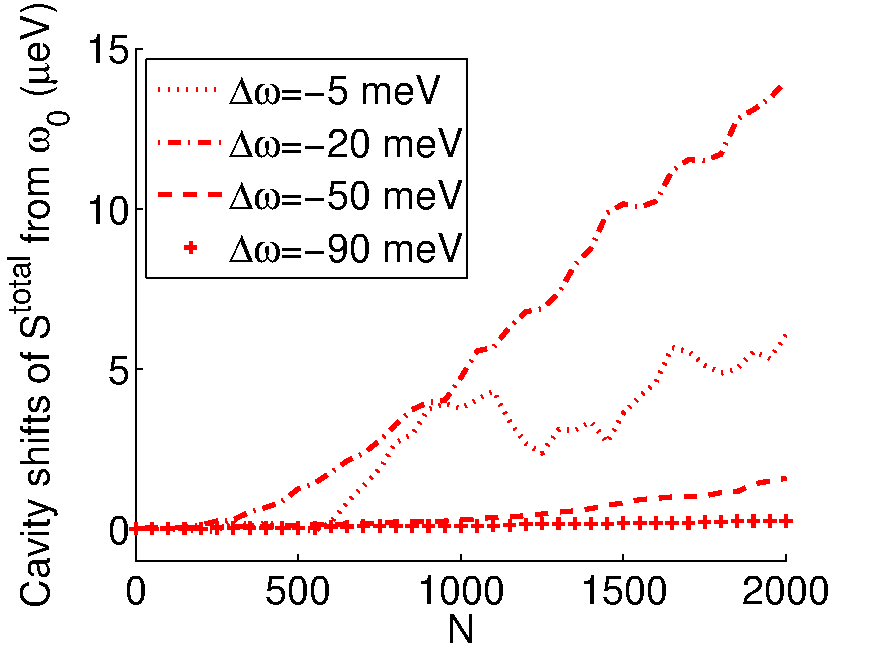
\includegraphics[width=0.33\textwidth]{./Figs/Stotalshift_wdrand5-90s20_gt0dot02b0dot5_qd2000_stat200}
    \label{Stotalshift_wdrand5-90s20_gt0.02b0.5_qd2000_stat200}}
%  \\
 \end{tabular}
\
  \begin{tabular}{cc}
  \subfigure[ ]{
    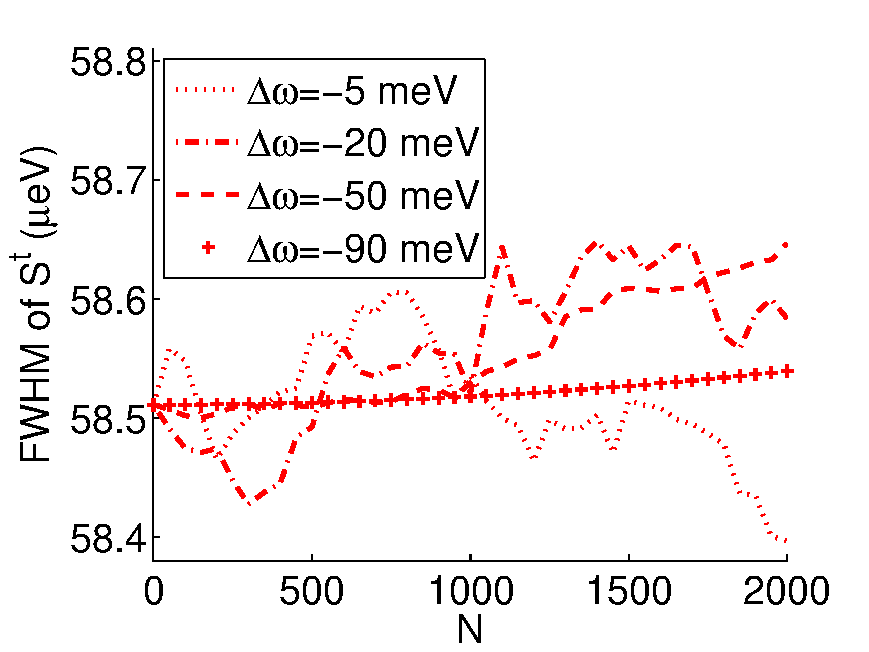
\includegraphics[width=0.33\textwidth]{./Figs/Stfwhm_wdrand5-90s20_gt0dot02b0dot5_qd2000_stat200}
    \label{Stfwhm_wdrand5-90s20_gt0.02b0.5_qd2000_stat200}}
  &
  \subfigure[ ]{
    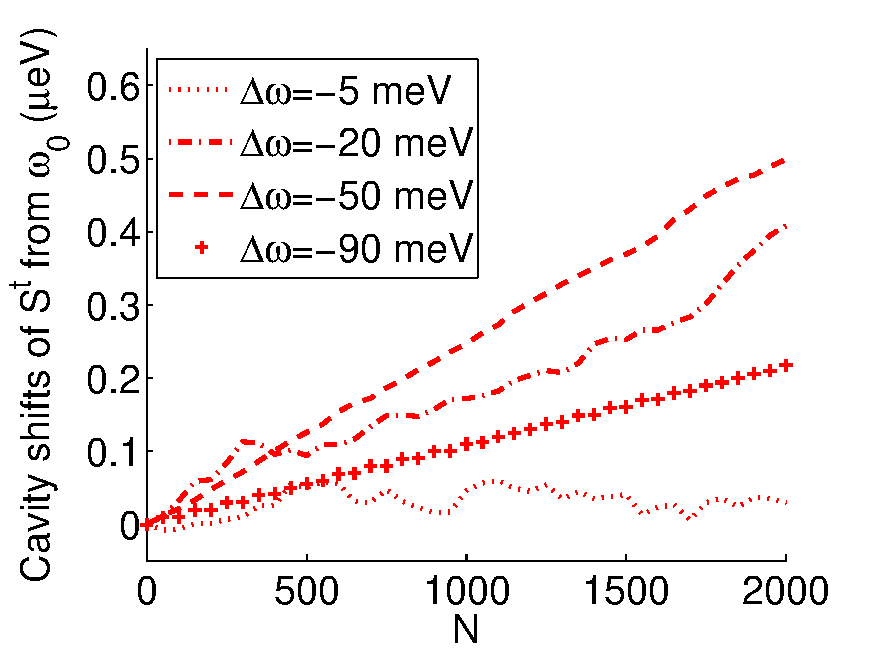
\includegraphics[width=0.33\textwidth]{./Figs/Stshift_wdrand5-90s20_gt0dot02b0dot5_qd2000_stat200}
    \label{Stshift_wdrand5-90s20_gt0.02b0.5_qd2000_stat200}}
\end{tabular}
\caption[Modification effect of different $\Delta\omega$ when $g_t=0.02$ meV.]{\textbf{FWHMs and shifts of the cavity and the target dipole spectra with different $\Delta\omega$ but with the same $g_t=0.02$ meV.} \subref{Stotalfwhm_wdrand5-90s20_gt0.02b0.5_qd2000_stat200} and \subref{Stotalshift_wdrand5-90s20_gt0.02b0.5_qd2000_stat200} show the total spectra are greatly broadened and shifted with the effect of close dipoles. The fluctuation feature is interpreted in the text, when $\Delta\omega$ is small. \subref{Stfwhm_wdrand5-90s20_gt0.02b0.5_qd2000_stat200} and \subref{Stshift_wdrand5-90s20_gt0.02b0.5_qd2000_stat200} show the similar effects on the target dipole spectra, but with a screening effect from the cavity peak. To demonstrate the phase retardation, we have averaged 600 samples for the four subfigures, and used a frequency domain resolution of $0.01\,\mu$eV for \subref{Stfwhm_wdrand5-90s20_gt0.02b0.5_qd2000_stat200} and \subref{Stshift_wdrand5-90s20_gt0.02b0.5_qd2000_stat200}, and $0.075\,\mu$eV for \subref{Stotalfwhm_wdrand5-90s20_gt0.02b0.5_qd2000_stat200} and \subref{Stotalshift_wdrand5-90s20_gt0.02b0.5_qd2000_stat200}. }
\label{fwhm_shift_gt0.02_dw}
\end{figure}
\end{frame}


\begin{frame}{Case 2: $ g_t=2g_b=0.04 $meV, changing $ \Delta\omega $.}
\begin{figure}[H]%[floatfix]
\centering
\begin{tabular}{cc}
  \subfigure[ ]{
    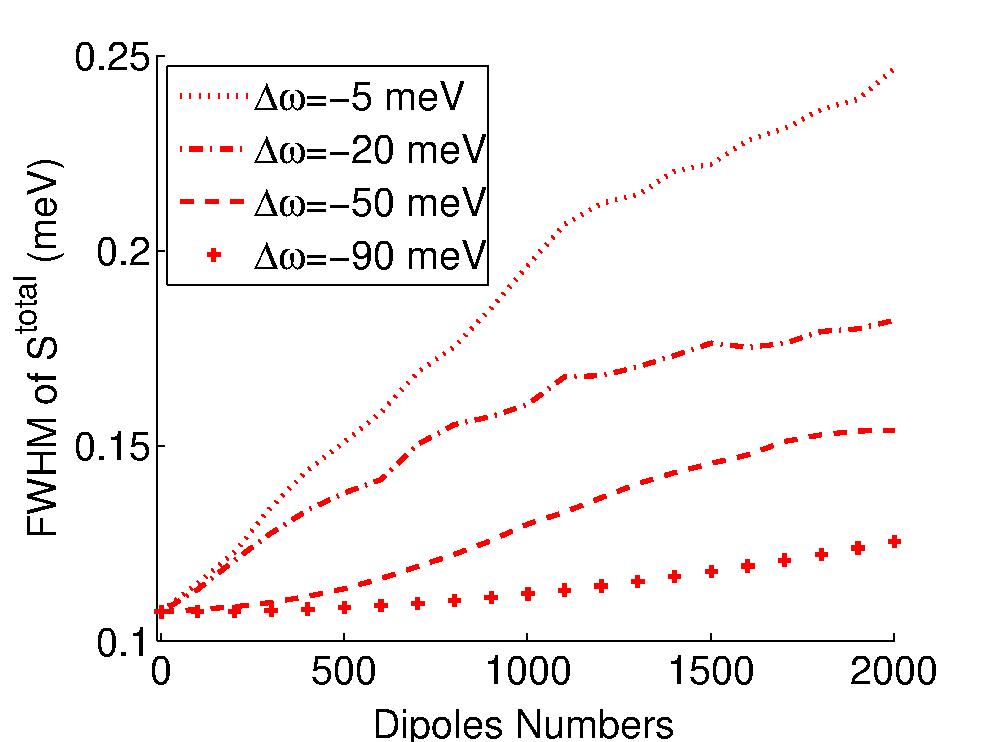
\includegraphics[width=0.33\textwidth]{./Figs/Stotalfwhm_wdrand5-90s20_gt0dot04b0dot5_qd2000_stat200}
    \label{Stotalfwhm_wdrand5-90s20_gt0.04b0.5_qd2000_stat200}}
  &
  \subfigure[ ]{
    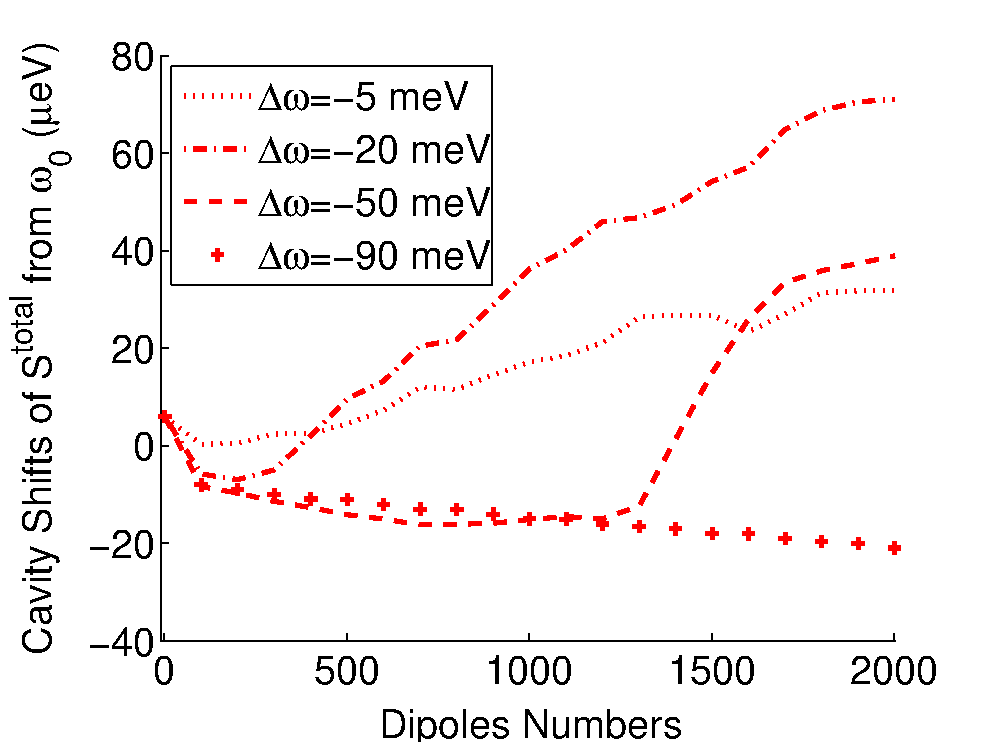
\includegraphics[width=0.33\textwidth]{./Figs/Stotalshift_wdrand5-90s20_gt0dot04b0dot5_qd2000_stat200}
    \label{Stotalshift_wdrand5-90s20_gt0.04b0.5_qd2000_stat200}}
  \\
  \subfigure[ ]{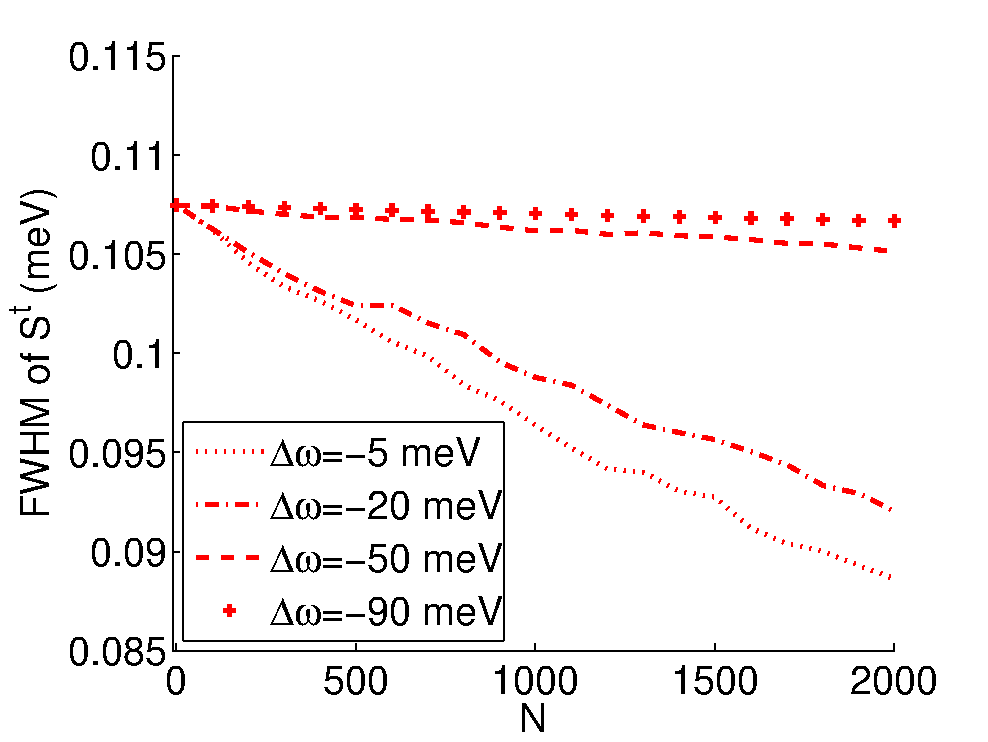
\includegraphics[width=0.33\textwidth]{./Figs/Stfwhm_wdrand5-90s20_gt0dot04b0dot5_qd2000_stat200}
    \label{Stfwhm_wdrand5-90s20_gt0.04b0.5_qd2000_stat200}}
  &
  \subfigure[ ]{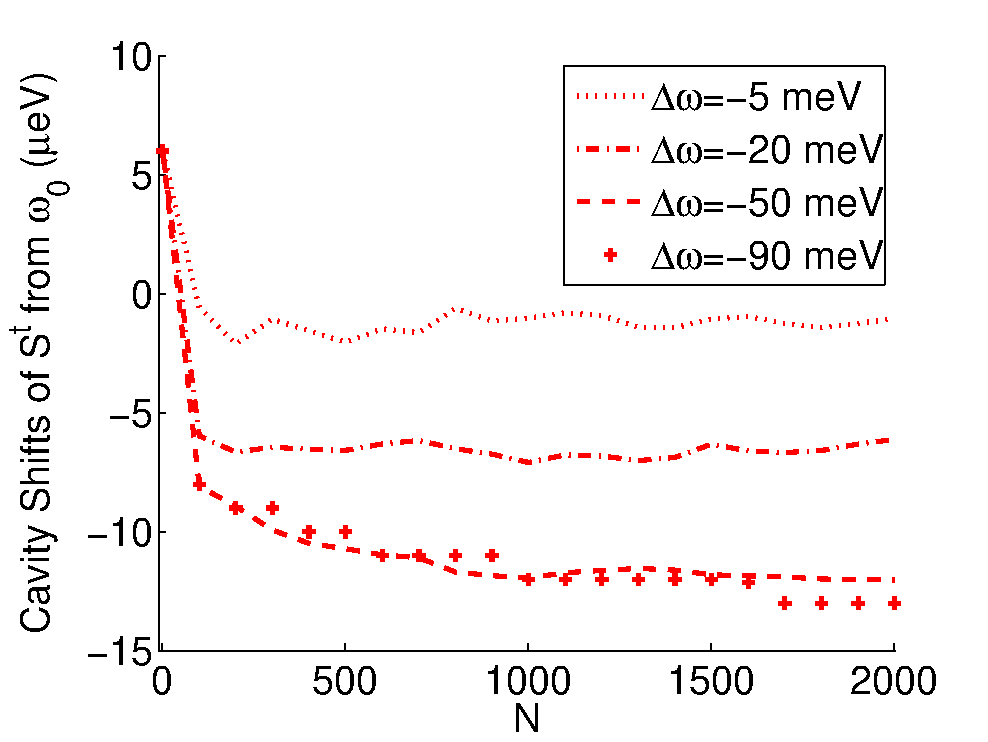
\includegraphics[width=0.33\textwidth]{./Figs/Stshift_wdrand5-90s20_gt0dot04b0dot5_qd2000_stat200}
    \label{Stshift_wdrand5-90s20_gt0.04b0.5_qd2000_stat200}}
\end{tabular}
\caption[Modification effect of different $\Delta\omega$ when $g_t=0.04$ meV.]{\textbf{FWHM and shifts of the cavity with different $\Delta\omega$ with the same $g_t=0.04$ meV.} As the doublets occur, the repulsion between doublets gives a different spectral behavior from what has been shown in Fig.~\ref{fwhm_shift_gt0.02_dw}. See text for the discussion.}
\label{fwhm_shift_gt0.04_dw}
\end{figure}
\end{frame}


\begin{frame}{Case 2: $ g_t=2g_b=0.04 $meV, changing $ \Delta\omega $.}

\begin{figure}[thp]%[floatfix]
\centering
\begin{center}
%\psfrag{PL}{$PL (to Max)$}
%\psfrag{omega-omega}{$\omega-\omega_c (meV)$}
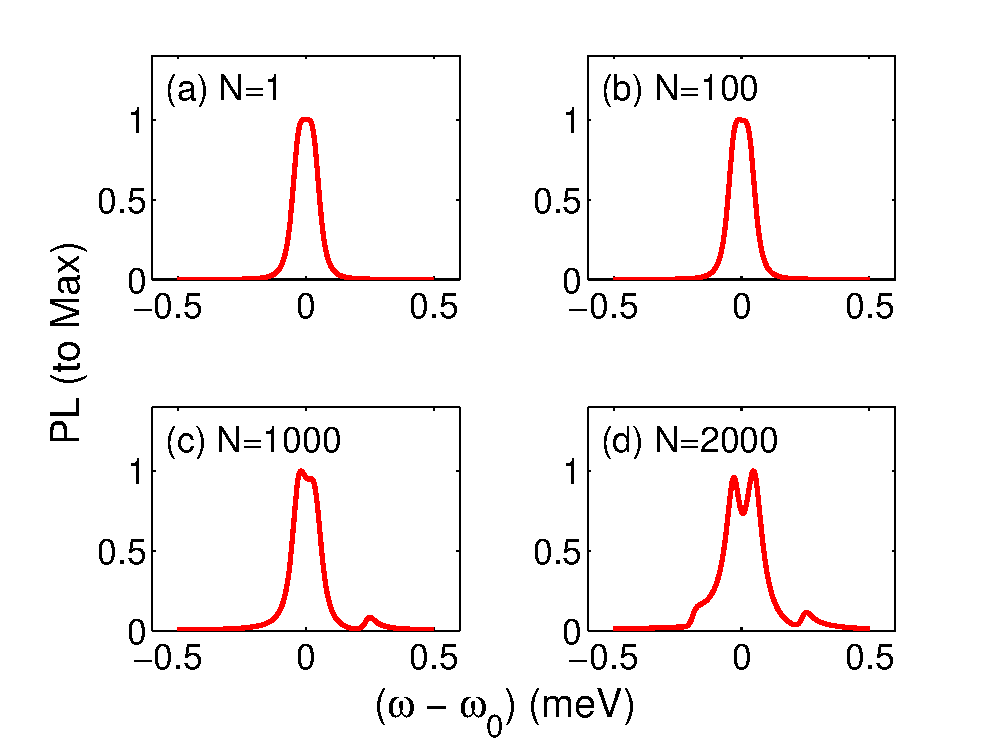
\includegraphics[width=0.72\textwidth]{./Figs/spec1tNb_wd50s20_gt0dot04E0dot5_stat200} %spec_wdrand5s20_E0.2_qd2000_stat200_sam32.eps
\end{center}
\caption[Spectra sample for a cavity with a target dipole and an ensemble.]{\fontsize{8}{0.2}\selectfont Cavity spectra of one set of dipoles sample ($\Delta\omega=-50$ meV, $\sigma=20$ meV) with various background dipole population $N$. 
%Doublets occur even though $g_t<0.5$ meV, which is the criterion of strong coupling for one-exciton cases.
}
\label{spec1tNb_wd50s20_gt0.04E0.5_stat200}
\end{figure}
\end{frame}


\begin{frame}{Summary of Cavity-exciton interaction}
\begin{columns}
\column{0.6\textwidth}
\begin{figure}[thp]%[floatfix]
\centering
\begin{center}
%\psfrag{PL}{$PL (to Max)$}
%\psfrag{omega-omega}{$\omega-\omega_c (meV)$}
\includegraphics[width=0.95\textwidth]{./Figs/Cavity_BackgroundDipoles_TargetDipole} %spec_wdrand5s20_E0.2_qd2000_stat200_sam32.eps
\end{center}
\caption[Cavity and exciton ensemble interaction.]{\fontsize{8}{0.2}\selectfont Cavity and exciton ensemble interactions. 
%Doublets occur even though $g_t<0.5$ meV, which is the criterion of strong coupling for one-exciton cases.
}
\end{figure}
\column{0.4\textwidth}
\fontsize{8}{0.2}\selectfont
\begin{itemize}
\item Background excitons and target excitons
\item On/Off-resonance
\item Frequencies Repulsion and Normal Broadening effects
\end{itemize}
\end{columns}
\end{frame}


\section{Future Work}

\begin{frame}{Essentials of GF Method}
\begin{itemize}
  \item
    \alert{What GF method can do?}
    \begin{itemize}
        \item
          Collective emission and interactions.
        \item
          In arbitrary optical structures.
     \end{itemize}
     \pause
  \item
    \alert{Limitations:}
    \begin{itemize}
        \item
          No dephasing, no decoherence.
        \item
          Works in linear or weak excitation regime.
     \end{itemize}
  \end{itemize}

\end{frame}

\begin{frame}{Possible Future Researches}
\begin{itemize}
  \item
    \alert{Neutral atoms in photonical structures}
    \begin{itemize}
        \item
          Polarization control for quantum computation.
        \item
          Backaction and forward propagation of light.
        \item
          Photon Anti-bunching...
     \end{itemize}
  \item
    \alert{Other areas:}
    \begin{itemize}
        \item
          QDs $+$ waveguide, etc.
        \item
          NV centers in a diamond...
     \end{itemize}
\end{itemize}


\end{frame}





\section*{Summary}

\begin{frame}{Summary}

  % Keep the summary *very short*.
  \begin{itemize}
  \item
    A theory of light-ensemble interaction.
  \item
    Green function method in nanophotonics and quantum optics.
  \item
    Applications: pumping dynamics, frequencies repulsion and spectral broadening...
  \item 
    Future work.
  \end{itemize}
  
%  % The following outlook is optional.
%  \vskip0pt plus.5fill
%  \begin{itemize}
%  \item
%    Outlook
%    \begin{itemize}
%    \item
%      Something you haven't solved.
%    \item
%      Something else you haven't solved.
%    \end{itemize}
%  \end{itemize}
\end{frame}

\begin{frame}{}
\begin{center}
  \Large \textbf{Questions?}
  
  \vskip15pt
  \vskip15pt
  \vskip10pt
  
  \Large \textbf{Thank You!}
\end{center}
\end{frame}



% All of the following is optional and typically not needed. 
\appendix
\section<presentation>*{\appendixname}
\subsection<presentation>*{For Further Reading}

\begin{frame}[allowframebreaks]
  \frametitle<presentation>{For Further Reading}
    
%  \begin{thebibliography}{10}
%    
%  \beamertemplatebookbibitems
%  % Start with overview books.
%
%  \bibitem{Author1990}
%    A.~Author.
%    \newblock {\em Handbook of Everything}.
%    \newblock Some Press, 1990.
% 
%    
%  \beamertemplatearticlebibitems
%  % Followed by interesting articles. Keep the list short. 
%
%  \bibitem{Someone2000}
%    S.~Someone.
%    \newblock On this and that.
%    \newblock {\em Journal of This and That}, 2(1):50--100,
%    2000.
%  \end{thebibliography}
\end{frame}

%\begin{frame}
%\bibliographystyle{unsrt}
%\bibliography{F:/References/HughesGroup/Queen}
%%\bibliography{E:/References/Queens/Queen}
%\end{frame}
\end{document}


